\chapter{Diboson studies}
\label{chap:dibosons}

In dark matter searches involving a Z boson in the final state, 
the resonant diboson processes $\Z\Z$ and $\W\Z$ are an irreducible background.
In the case of hadronic Z boson decays, they are not a major worry, since
other hadronic background processes such as pure QCD totally beat out the
diboson processes based on the cross-sections \cite{Sirunyan:2017jix}.
On the other hand, in final states with little hadronic activity,
the other background processes which contribute substantially are easy to reject.
These diboson processes quickly become the main problem due to our limited theoretical understanding of them.

In this chapter, I survey the current status of theoretical calculations for dibosons. 
Then, I discuss two separate analysis selections to obtain pure control samples 
of the ZZ and WZ processes.
These data are interesting on their own to compare to the simulation as a precision electroweak measurement.
In the context of this work, they are also a crucial ingredient
for the dark matter search of Chapter~\ref{chap:zlldm}.

\section{Limitations of simulating diboson processes}
\label{sec:vvtheo}
All simulated physics processes in this work are susceptible to uncertainties due to: the proton parton distribution functions; the QCD scale, $\alpha_s$; and the renormalization and factorization scales in the quantum field theory.
Consistent with the other processes, these effects are propagated to both the overall cross sections and the transverse momentum spectra of the $\Z\Z$ and $\W\Z$ processes.
For the purposes of motivating this chapter, it suffices to say that the effect of these is roughly 10\%. 

Meanwhile, as previously outlined in \ref{sec:higher-order-corrections}, the endgame-level precision for the $\Z\Z$ and $\W\Z$ simulations is NNLO in QCD and NLO in electroweak.
Since no cohesive theoretical calculation is available at this level of precision, our duct-tape assembly of higher-order corrections come at a price.
Namely, the contribution from diagrams at NLO in both QCD and electroweak is ignored. Thus arises the so-called ``QCD-electroweak cross-term.''

\begin{figure}[hb] % ZZ
 \centering
 \begin{tikzpicture} % ZZ to 4l LO
  \begin{feynman}
   \vertex (q1) {\(\boldsymbol{\Pq}\)};
   \vertex [below= 2cm of q1] (q2) {\(\boldsymbol{\Paq}\)};
   \vertex [right= 2cm of q1] (a);
   \vertex [right= 2cm of q2] (b);
   \vertex [right= 2cm of a] (c);
   \vertex [right= 2cm of b] (d);
   \vertex [right= 1.5cm of c] (e);
   \vertex [right= 1.5cm of d] (f);
   \vertex [above= 0.3cm of e] (f1) {\(\boldsymbol{\ell}\)};
   \vertex [below= 0.3cm of e] (f2) {\(\boldsymbol{\bar{\ell}}\)};
   \vertex [above= 0.3cm of f] (f3) {\(\boldsymbol{\ell}\)};
   \vertex [below= 0.3cm of f] (f4) {\(\boldsymbol{\bar{\ell}}\)};
   
   \diagram* {
    (q1) -- [fermion, very thick] (a),
    (q2) -- [anti fermion, very thick] (b),
    (a) -- [fermion, very thick] (b),
    (a) -- [boson, very thick, edge label'=\(\boldsymbol{\Z}\)] (c),
    (b) -- [boson, very thick, edge label'=\(\boldsymbol{\Z}\)] (d),
    (c) -- [fermion, very thick] (f1),
    (c) -- [anti fermion, very thick] (f2),
    (d) -- [fermion, very thick] (f3),
    (d) -- [anti fermion, very thick] (f4),
   };
  \end{feynman}
 \end{tikzpicture} \hspace{1cm}
 \begin{tikzpicture} %% ZZ to 4l NLO QCD
  \begin{feynman}
   \vertex (q1) {\(\boldsymbol{\Pq}\)};
   \vertex [below= 2cm of q1] (q2) {\(\boldsymbol{\Paq}\)};
   \vertex [right= 2cm of q1] (a);
   \vertex [right= 2cm of q2] (b);
   \vertex [right= 2cm of a] (c);
   \vertex [right= 2cm of b] (d);
   \vertex [right= 1.5cm of c] (e);
   \vertex [right= 1.5cm of d] (f);
   \vertex [above= 0.3cm of e] (f1) {\(\boldsymbol{\ell}\)};
   \vertex [below= 0.3cm of e] (f2) {\(\boldsymbol{\bar{\ell}}\)};
   \vertex [above= 0.3cm of f] (f3) {\(\boldsymbol{\ell}\)};
   \vertex [below= 0.3cm of f] (f4) {\(\boldsymbol{\bar{\ell}}\)};
   \vertex [right= 0.8cm of q1] (g1);
   \vertex [below= 0.7cm of a] (g2);
   
   \diagram* {
    (q1) -- [fermion, very thick] (a),
    (q2) -- [anti fermion, very thick] (b),
    (a) -- [fermion, very thick] (b),
    (a) -- [boson, very thick, edge label'=\(\boldsymbol{\Z}\)] (c),
    (b) -- [boson, very thick, edge label'=\(\boldsymbol{\Z}\)] (d),
    (c) -- [fermion, very thick] (f1),
    (c) -- [anti fermion, very thick] (f2),
    (d) -- [fermion, very thick] (f3),
    (d) -- [anti fermion, very thick] (f4),
    (g1) -- [gluon, very thick, bend right, edge label'=\(\boldsymbol{g}\)] (g2),
   };
  \end{feynman}
 \end{tikzpicture}  \vspace{1cm}
 
 \begin{tikzpicture} %% ZZ to 4l NLO only EW
  \begin{feynman}
   \vertex (q1) {\(\boldsymbol{\Pq}\)};
   \vertex [below= 2cm of q1] (q2) {\(\boldsymbol{\Paq}\)};
   \vertex [right= 2cm of q1] (a);
   \vertex [right= 2cm of q2] (b);
   \vertex [right= 2cm of a] (c);
   \vertex [right= 2cm of b] (d);
   \vertex [right= 1.5cm of c] (e);
   \vertex [right= 1.5cm of d] (f);
   \vertex [above= 0.3cm of e] (f1) {\(\boldsymbol{\ell}\)};
   \vertex [below= 0.3cm of e] (f2) {\(\boldsymbol{\bar{\ell}}\)};
   \vertex [above= 0.3cm of f] (f3) {\(\boldsymbol{\ell}\)};
   \vertex [below= 0.3cm of f] (f4) {\(\boldsymbol{\bar{\ell}}\)};
   \vertex [right= 0.8cm of q2] (V1);
   \vertex [above= 0.7cm of b] (V2);
   
   \diagram* {
    (q1) -- [fermion, very thick] (a),
    (q2) -- [anti fermion, very thick] (b),
    (a) -- [fermion, very thick] (b),
    (a) -- [boson, very thick, edge label'=\(\boldsymbol{\Z}\)] (c),
    (b) -- [boson, very thick, edge label'=\(\boldsymbol{\Z}\)] (d),
    (c) -- [fermion, very thick] (f1),
    (c) -- [anti fermion, very thick] (f2),
    (d) -- [fermion, very thick] (f3),
    (d) -- [anti fermion, very thick] (f4),
    (V1) -- [boson, very thick, bend left, edge label=\(\boldsymbol{\Z/\W/\gamma}\)] (V2),
   };
  \end{feynman}
 \end{tikzpicture} \hspace{1cm}
 \begin{tikzpicture} %% ZZ to 4l NLO EW and QCD
  \begin{feynman}
   \vertex (q1) {\(\boldsymbol{\Pq}\)};
   \vertex [below= 2cm of q1] (q2) {\(\boldsymbol{\Paq}\)};
   \vertex [right= 2cm of q1] (a);
   \vertex [right= 2cm of q2] (b);
   \vertex [right= 2cm of a] (c);
   \vertex [right= 2cm of b] (d);
   \vertex [right= 1.5cm of c] (e);
   \vertex [right= 1.5cm of d] (f);
   \vertex [above= 0.3cm of e] (f1) {\(\boldsymbol{\ell}\)};
   \vertex [below= 0.3cm of e] (f2) {\(\boldsymbol{\bar{\ell}}\)};
   \vertex [above= 0.3cm of f] (f3) {\(\boldsymbol{\ell}\)};
   \vertex [below= 0.3cm of f] (f4) {\(\boldsymbol{\bar{\ell}}\)};
   \vertex [right= 0.8cm of q1] (V1);
   \vertex [below= 0.7cm of a] (V2);
   \vertex [right= 1.2cm of q2] (g1);
   \vertex [below= 1cm of g1] (g2);
   \vertex [right= 1.3cm of g2] (g3);
   
   \diagram* {
    (q1) -- [fermion, very thick] (a),
    (q2) -- [anti fermion, very thick] (b),
    (a) -- [fermion, very thick] (b),
    (a) -- [boson, very thick, edge label'=\(\boldsymbol{\Z}\)] (c),
    (b) -- [boson, very thick, edge label'=\(\boldsymbol{\Z}\)] (d),
    (c) -- [fermion, very thick] (f1),
    (c) -- [anti fermion, very thick] (f2),
    (d) -- [fermion, very thick] (f3),
    (d) -- [anti fermion, very thick] (f4),
    (V1) -- [boson, very thick, bend right, edge label'=\(\boldsymbol{\Z/\W/\gamma}\)] (V2),
    (g1) -- [gluon, very thick, edge label'=\(\boldsymbol{g}\)] (g3),
   };
  \end{feynman}
 \end{tikzpicture}

 \caption{Clockwise from upper left: ZZ production at leading order; ZZ production at NLO in QCD; ZZ production at NLO in both QCD and EW; ZZ production at NLO only in EW.} \label{fig:ZZto4l}
\end{figure}

The overall electroweak NLO correction to the $\W\Z$ process is relatively small, since the virtual corrections and photon-induced corrections partially cancel.
Therefore, the NLO QCD-electroweak cross-term for the $\W\Z$ process is also small.
On the other hand, the electroweak NLO corrections to the $\Z\Z$ process are large and momentum-dependent.
They bring a 10\% net reduction of the overall $\Z\Z$ yield, with a strong dependence on the lesser boson $p_\mathrm{T}$.
The $\met$ spectrum becomes much softer, with a correction of around $-40\%$ at lesser Z boson $p_\mathrm{T}$ of $700 \GeV$.
For this reason, the QCD-electroweak cross-term cannot be neglected for the $\Z\Z$ process, and a conservative
assessment of this missing term gives an overall effect of roughly $25\%$.

\begin{figure}[hb] % WZ
 \centering
 \begin{tikzpicture} % WZ at LO (s-channel)
  \begin{feynman}
   \vertex (q1) {\(\boldsymbol{\Pq}\)};
   \vertex [below= 3cm of q1] (q2) {\(\boldsymbol{\Paq'}\)};
   \vertex [right= 1.6cm of q1] (a1);
   \vertex [below= 1.5cm of a1] (a2);
   \vertex [right= 1.6cm of a2] (b1);
   \vertex [right= 1.6cm of b1] (c1);
   \vertex [above= 1.3cm of c1] (c2);
   \vertex [below= 1.3cm of c1] (c3);
   \vertex [right= 1cm of c2] (d1);
   \vertex [right= 1cm of c3] (d2);
   \vertex [above= 0.3cm of d1] (f1) {\(\boldsymbol{\ell}\)};
   \vertex [below= 0.3cm of d1] (f2) {\(\boldsymbol{\bar{\ell}}\)};
   \vertex [above= 0.3cm of d2] (f3) {\(\boldsymbol{\ell}\)};
   \vertex [below= 0.3cm of d2] (f4) {\(\boldsymbol{\bar{\nu_\ell}}\)};
   
   \diagram* {
    (q1) -- [fermion, very thick] (a2),
    (q2) -- [anti fermion, very thick] (a2),
    (a2) -- [boson, very thick, edge label'=\(\boldsymbol{\PWm}\)] (b1),
    (b1) -- [boson, very thick, edge label=\(\boldsymbol{\Z}\)] (c2),
    (b1) -- [boson, very thick, edge label=\(\boldsymbol{\PWm}\)] (c3),
    (c2) -- [fermion, very thick] (f1),
    (c2) -- [anti fermion, very thick] (f2),
    (c3) -- [fermion, very thick] (f3),
    (c3) -- [anti fermion, very thick] (f4),
   };
  \end{feynman}
 \end{tikzpicture} \hspace{1cm}
 \begin{tikzpicture} % WZ at LO (t-channel)
  \begin{feynman}
   \vertex (q1) {\(\boldsymbol{\Pq}\)};
   \vertex [below= 2cm of q1] (q2) {\(\boldsymbol{\Paq'}\)};
   \vertex [right= 2cm of q1] (a);
   \vertex [right= 2cm of q2] (b);
   \vertex [right= 2cm of a] (c);
   \vertex [right= 2cm of b] (d);
   \vertex [right= 1.5cm of c] (e);
   \vertex [right= 1.5cm of d] (f);
   \vertex [above= 0.3cm of e] (f1) {\(\boldsymbol{\ell}\)};
   \vertex [below= 0.3cm of e] (f2) {\(\boldsymbol{\bar{\ell}}\)};
   \vertex [above= 0.3cm of f] (f3) {\(\boldsymbol{\nu_\ell}\)};
   \vertex [below= 0.3cm of f] (f4) {\(\boldsymbol{\bar{\ell}}\)};
   
   \diagram* {
    (q1) -- [fermion, very thick] (a),
    (q2) -- [anti fermion, very thick] (b),
    (a) -- [fermion, very thick] (b),
    (a) -- [boson, very thick, edge label'=\(\boldsymbol{\Z}\)] (c),
    (b) -- [boson, very thick, edge label'=\(\boldsymbol{\PWp}\)] (d),
    (c) -- [fermion, very thick] (f1),
    (c) -- [anti fermion, very thick] (f2),
    (d) -- [fermion, very thick] (f3),
    (d) -- [anti fermion, very thick] (f4),
   };
  \end{feynman}
 \end{tikzpicture}  
 \caption{Leading order WZ production mechanisms in the $s$-channel and the $t$-channel.} \label{fig:WZLO}
\end{figure}

\begin{figure}[hb] % WZ NLO EW
 \centering
 \begin{tikzpicture} % WZ at NLO EW (s-channel) internal loop
  \begin{feynman}
   \vertex (q1) {\(\boldsymbol{\Pq}\)};
   \vertex [below= 3cm of q1] (q2) {\(\boldsymbol{\Paq'}\)};
   \vertex [right= 1.5cm of q1] (a1);
   \vertex [below= 1.5cm of a1] (a2);
   \vertex [right= 1.6cm of a2] (b1);
   \vertex [right= 1.6cm of b1] (c1);
   \vertex [above= 1.3cm of c1] (c2);
   \vertex [below= 1.3cm of c1] (c3);
   \vertex [right= 1cm of c2] (d1);
   \vertex [right= 1cm of c3] (d2);
   \vertex [above= 0.3cm of d1] (f1) {\(\boldsymbol{\ell}\)};
   \vertex [below= 0.3cm of d1] (f2) {\(\boldsymbol{\bar{\ell}}\)};
   \vertex [above= 0.3cm of d2] (f3) {\(\boldsymbol{\ell}\)};
   \vertex [below= 0.3cm of d2] (f4) {\(\boldsymbol{\bar{\nu_\ell}}\)};
   \vertex [below right= 0.9cm of q1] (V1);
   \vertex [above right= 0.9cm of q2] (V2);
   
   \diagram* {
    (q1) -- [fermion, very thick] (a2),
    (q2) -- [anti fermion, very thick] (a2),
    (a2) -- [boson, very thick, edge label'=\(\boldsymbol{\PWm}\)] (b1),
    (b1) -- [boson, very thick, edge label=\(\boldsymbol{\Z}\)] (c2),
    (b1) -- [boson, very thick, edge label=\(\boldsymbol{\PWm}\)] (c3),
    (c2) -- [fermion, very thick] (f1),
    (c2) -- [anti fermion, very thick] (f2),
    (c3) -- [fermion, very thick] (f3),
    (c3) -- [anti fermion, very thick] (f4),
    (V1) -- [boson, very thick, edge label'=\(\boldsymbol{\Z/\W/\gamma}\)] (V2),
   };
  \end{feynman}
 \end{tikzpicture} \hspace{1cm}
 \begin{tikzpicture} % WZ at NLO (t-channel) internal loop
  \begin{feynman}
   \vertex (q1) {\(\boldsymbol{\Pq}\)};
   \vertex [below= 2cm of q1] (q2) {\(\boldsymbol{\Paq'}\)};
   \vertex [right= 2cm of q1] (a);
   \vertex [right= 2cm of q2] (b);
   \vertex [right= 2cm of a] (c);
   \vertex [right= 2cm of b] (d);
   \vertex [right= 1.5cm of c] (e);
   \vertex [right= 1.5cm of d] (f);
   \vertex [above= 0.3cm of e] (f1) {\(\boldsymbol{\ell}\)};
   \vertex [below= 0.3cm of e] (f2) {\(\boldsymbol{\bar{\ell}}\)};
   \vertex [above= 0.3cm of f] (f3) {\(\boldsymbol{\nu_\ell}\)};
   \vertex [below= 0.3cm of f] (f4) {\(\boldsymbol{\bar{\ell}}\)};
   \vertex [right= 0.8cm of q2] (V1);
   \vertex [above= 0.7cm of b] (V2);
   
   \diagram* {
    (q1) -- [fermion, very thick] (a),
    (q2) -- [anti fermion, very thick] (b),
    (a) -- [fermion, very thick] (b),
    (a) -- [boson, very thick, edge label'=\(\boldsymbol{\Z}\)] (c),
    (b) -- [boson, very thick, edge label'=\(\boldsymbol{\W^+}\)] (d),
    (c) -- [fermion, very thick] (f1),
    (c) -- [anti fermion, very thick] (f2),
    (d) -- [fermion, very thick] (f3),
    (d) -- [anti fermion, very thick] (f4),
    (V1) -- [boson, very thick, bend left, edge label=\(\boldsymbol{\Z/\W/\gamma}\)] (V2),
   };
  \end{feynman}
 \end{tikzpicture} \vspace{1cm}

 \begin{tikzpicture} % WZ at NLO EW (s-channel) y-induced
  \begin{feynman}
   \vertex (y1) {\(\boldsymbol{\gamma}\)};
   \vertex [below= 3cm of y1] (q2) {\(\boldsymbol{\Pq}\)};
   \vertex [right= 1.5cm of q1] (a1);
   \vertex [below= 1.5cm of a1] (a2);
   \vertex [right= 1.6cm of a2] (b1);
   \vertex [right= 1.6cm of b1] (c1);
   \vertex [above= 1.3cm of c1] (c2);
   \vertex [below= 1.3cm of c1] (c3);
   \vertex [right= 1cm of c2] (d1);
   \vertex [right= 1cm of c3] (d2);
   \vertex [above= 0.3cm of d1] (f1) {\(\boldsymbol{\ell}\)};
   \vertex [below= 0.3cm of d1] (f2) {\(\boldsymbol{\bar{\ell}}\)};
   \vertex [above= 0.3cm of d2] (f3) {\(\boldsymbol{\ell}\)};
   \vertex [below= 0.3cm of d2] (f4) {\(\boldsymbol{\bar{\nu_\ell}}\)};
   \vertex [below right= 1.2cm of y1] (y2);
   \vertex [right= 1cm of y2] (fsrq1);
   \vertex [above= 0.6cm of fsrq1] (fsrq2) {\(\boldsymbol{\Pq'}\)};
   
   \diagram* {
    (y1) -- [boson, very thick] (y2),
    (y2) -- [anti fermion, very thick] (a2),
    (q2) -- [fermion, very thick] (a2),
    (a2) -- [boson, very thick, edge label'=\(\boldsymbol{\PWm}\)] (b1),
    (b1) -- [boson, very thick, edge label=\(\boldsymbol{\Z}\)] (c2),
    (b1) -- [boson, very thick, edge label=\(\boldsymbol{\PWm}\)] (c3),
    (c2) -- [fermion, very thick] (f1),
    (c2) -- [anti fermion, very thick] (f2),
    (c3) -- [fermion, very thick] (f3),
    (c3) -- [anti fermion, very thick] (f4),
    (y2) -- [fermion, very thick] (fsrq2),
   };
  \end{feynman}
 \end{tikzpicture} \hspace{1cm}
 \begin{tikzpicture} % WZ at NLO EW (t-channel) y-induced
  \begin{feynman}
   \vertex (y1) {\(\boldsymbol{\gamma}\)};
   \vertex [right= 1cm of y1] (y2);
   \vertex [below= 0.3cm of y2] (y3);
   \vertex [right= 1.8cm of y3] (fsrq1);
   \vertex [above= 0.2cm of fsrq1] (fsrq2) {\(\boldsymbol{\Pq'}\)};
   \vertex [below= 3.6cm of y1] (q2) {\(\boldsymbol{\Pq}\)};
   \vertex [right= 1cm of y3] (a1);
   \vertex [below= 0.5cm of a1] (a2);
   \vertex [right= 2cm of q2] (a3);
   \vertex [above= 0.8cm of a3] (a4);
   \vertex [right= 2cm of a2] (c);
   \vertex [right= 2cm of a4] (d);
   \vertex [right= 1.5cm of c] (e);
   \vertex [right= 1.5cm of d] (f);
   \vertex [above= 0.3cm of e] (f1) {\(\boldsymbol{\ell}\)};
   \vertex [below= 0.3cm of e] (f2) {\(\boldsymbol{\bar{\ell}}\)};
   \vertex [above= 0.3cm of f] (f3) {\(\boldsymbol{\nu_\ell}\)};
   \vertex [below= 0.3cm of f] (f4) {\(\boldsymbol{\bar{\ell}}\)};
   
   \diagram* {
    (y1) -- [boson, very thick] (y3),
    (y3) -- [anti fermion, very thick] (a2),
    (q2) -- [fermion, very thick] (a4),
    (a2) -- [anti fermion, very thick] (a4),
    (a2) -- [boson, very thick, edge label'=\(\boldsymbol{\Z}\)] (c),
    (a4) -- [boson, very thick, edge label'=\(\boldsymbol{\PWp}\)] (d),
    (c) -- [fermion, very thick] (f1),
    (c) -- [anti fermion, very thick] (f2),
    (d) -- [fermion, very thick] (f3),
    (d) -- [anti fermion, very thick] (f4),
    (y3) -- [fermion, very thick] (fsrq2),
   };
  \end{feynman}
 \end{tikzpicture}  
 

 \caption{WZ production at NLO in EW by internal loop processes (upper row) and photon-quark induced processes (lower row).} \label{fig:WZNLO}
\end{figure}

Yet another conservative step is taken regarding the NNLO QCD corrections.
For lack of a better method, the PDF and QCD scale uncertainties from the original POWHEG calculation at NLO in QCD are carried forward,
even though the final distributions are corrected to NNLO in QCD.
This represents another setback in the understanding of the diboson processes.

So far, in this chapter I have presented a bleak picture of the diboson calculations.
There is a silver lining to this: it is possible to control these cumbersome uncertainties by exploring the experimental data.
In the sections below are outlined two statistically independent control samples, with visible diboson events.

\clearpage
\section{ZZ process}
\label{sec:zz4l}
Here, I will describe how events are selected to observe the fully visible ZZ process.
Two Z boson candidates are each formed from a pair of opposite-charge electrons or muons having invariant mass within 15 \GeV of the Z boson mass resonance (91.1876 \GeV).
The Z candidate whose invariant mass is closer to the Z mass is denoted as $\mathrm{Z}_1$; the other, as $\mathrm{Z}_2$.
In total, there are four well-identified leptons, giving a very high purity selection.
Therefore neither hadronic $\tau$ nor b-jet vetoes are applied.
The minimum dilepton invariant mass, considering all pairs, must be greater than 4 \GeV.
The purpose of this is to reject the so-called ``nonprompt'' backgrounds, which I will explain next.

There is triboson contamination which is the resonant contribution from three bosons (WWZ, WZZ, ZZZ), or two top quarks and a Z boson.
There is also a small amount of contamination from the nonprompt backgrounds,
including but not limited to the Drell-Yan process, semileptonic diboson decays, leptonic WW decays, and ditop production.
From these, it is still possible to end up with four charged leptons or fake lepton signatures after the hard process.
These have been mostly suppressed by the minimum dilepton mass requirement.
Last but not least, there are Standard Model Higgs boson decays to four leptons
via $\mathrm{H}\rightarrow \mathrm{ZZ^*} \rightarrow 4\ell$, 
but the cross section is comparatively small.

The selection yields in simulation and data for this ZZ analysis are shown in Table~\ref{tab:zz4lyields}.
Distributions of illustrative variables after the selection are shown in Figures~\ref{fig:zz4l_mll},~\ref{fig:zz4l_zpt}, and~\ref{fig:zz4l_moreplots}.

\begin{figure}[!hb]
\centering
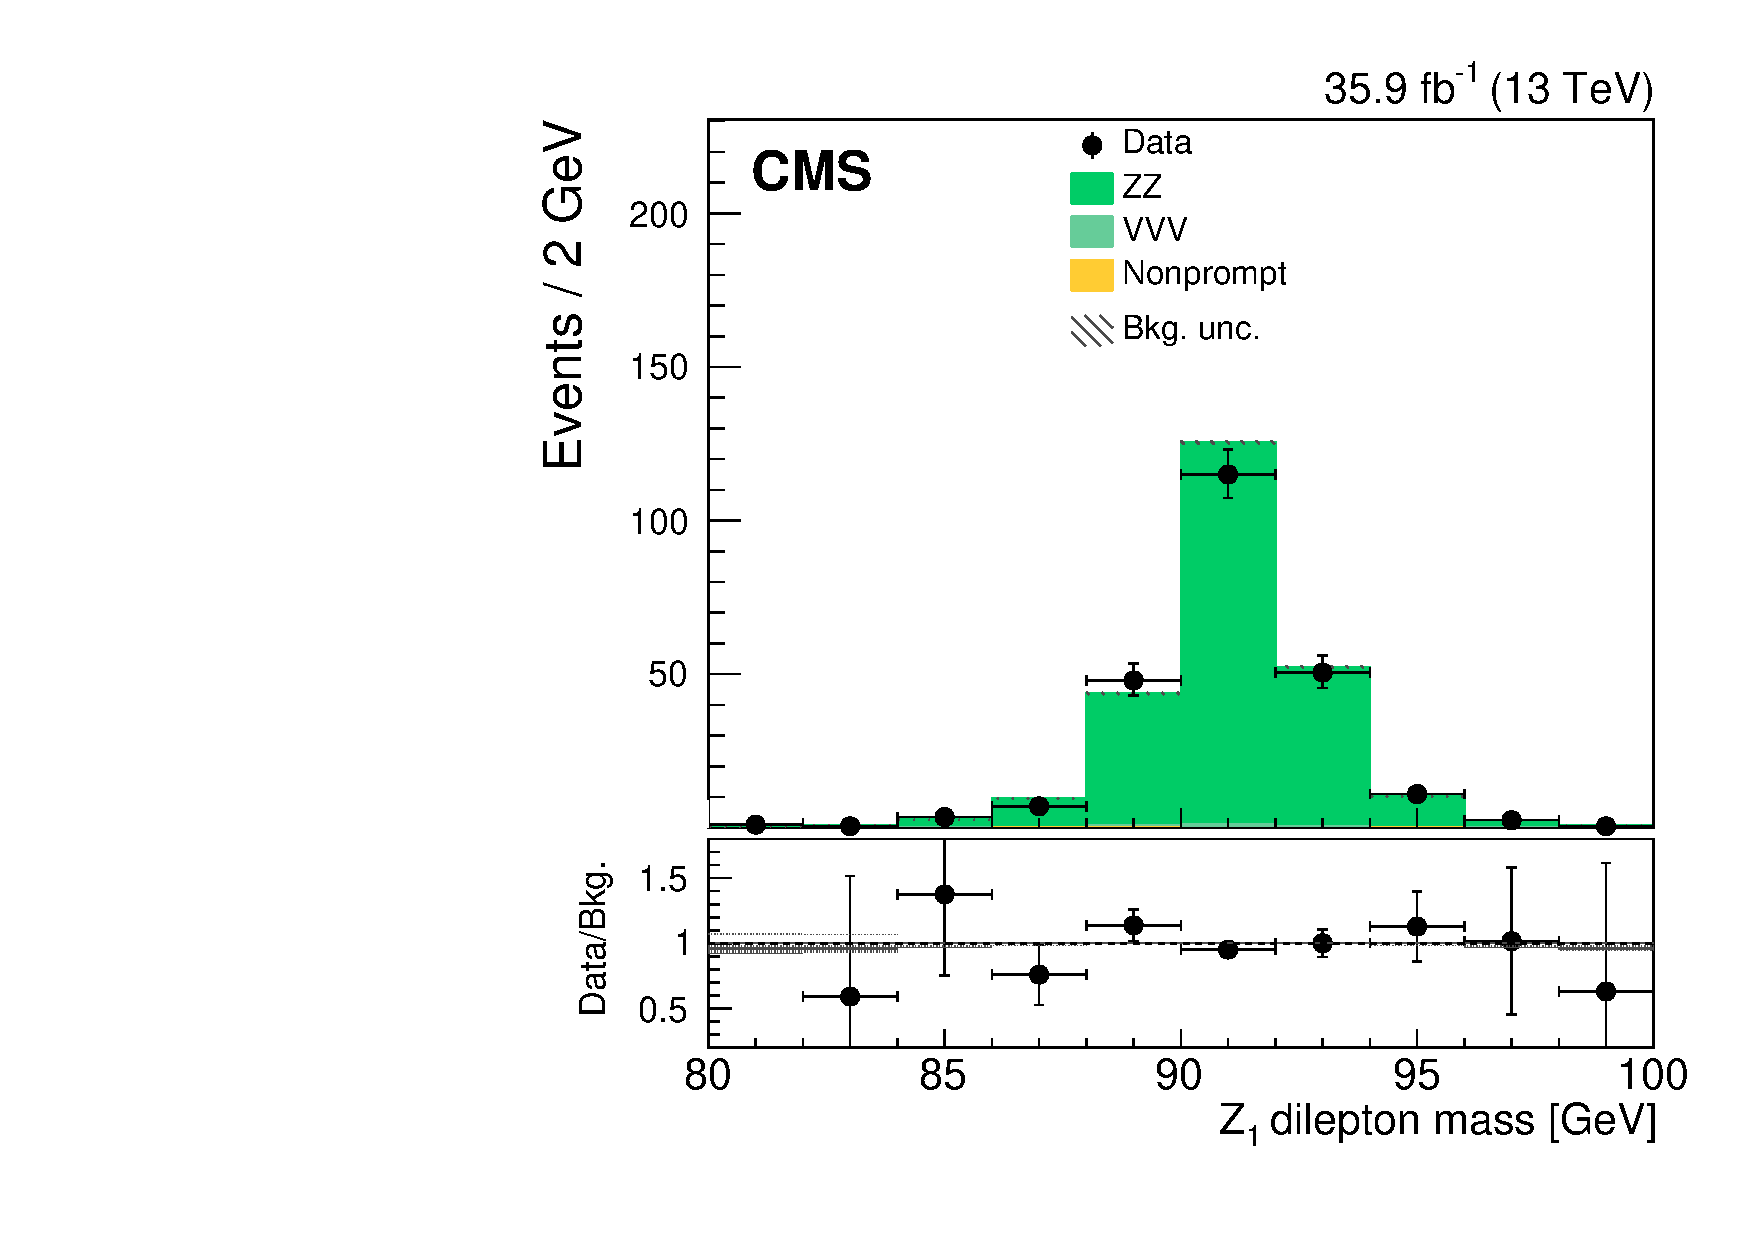
\includegraphics[width=0.48\textwidth]{figures/dibosons/zz4l/mZ1.pdf}
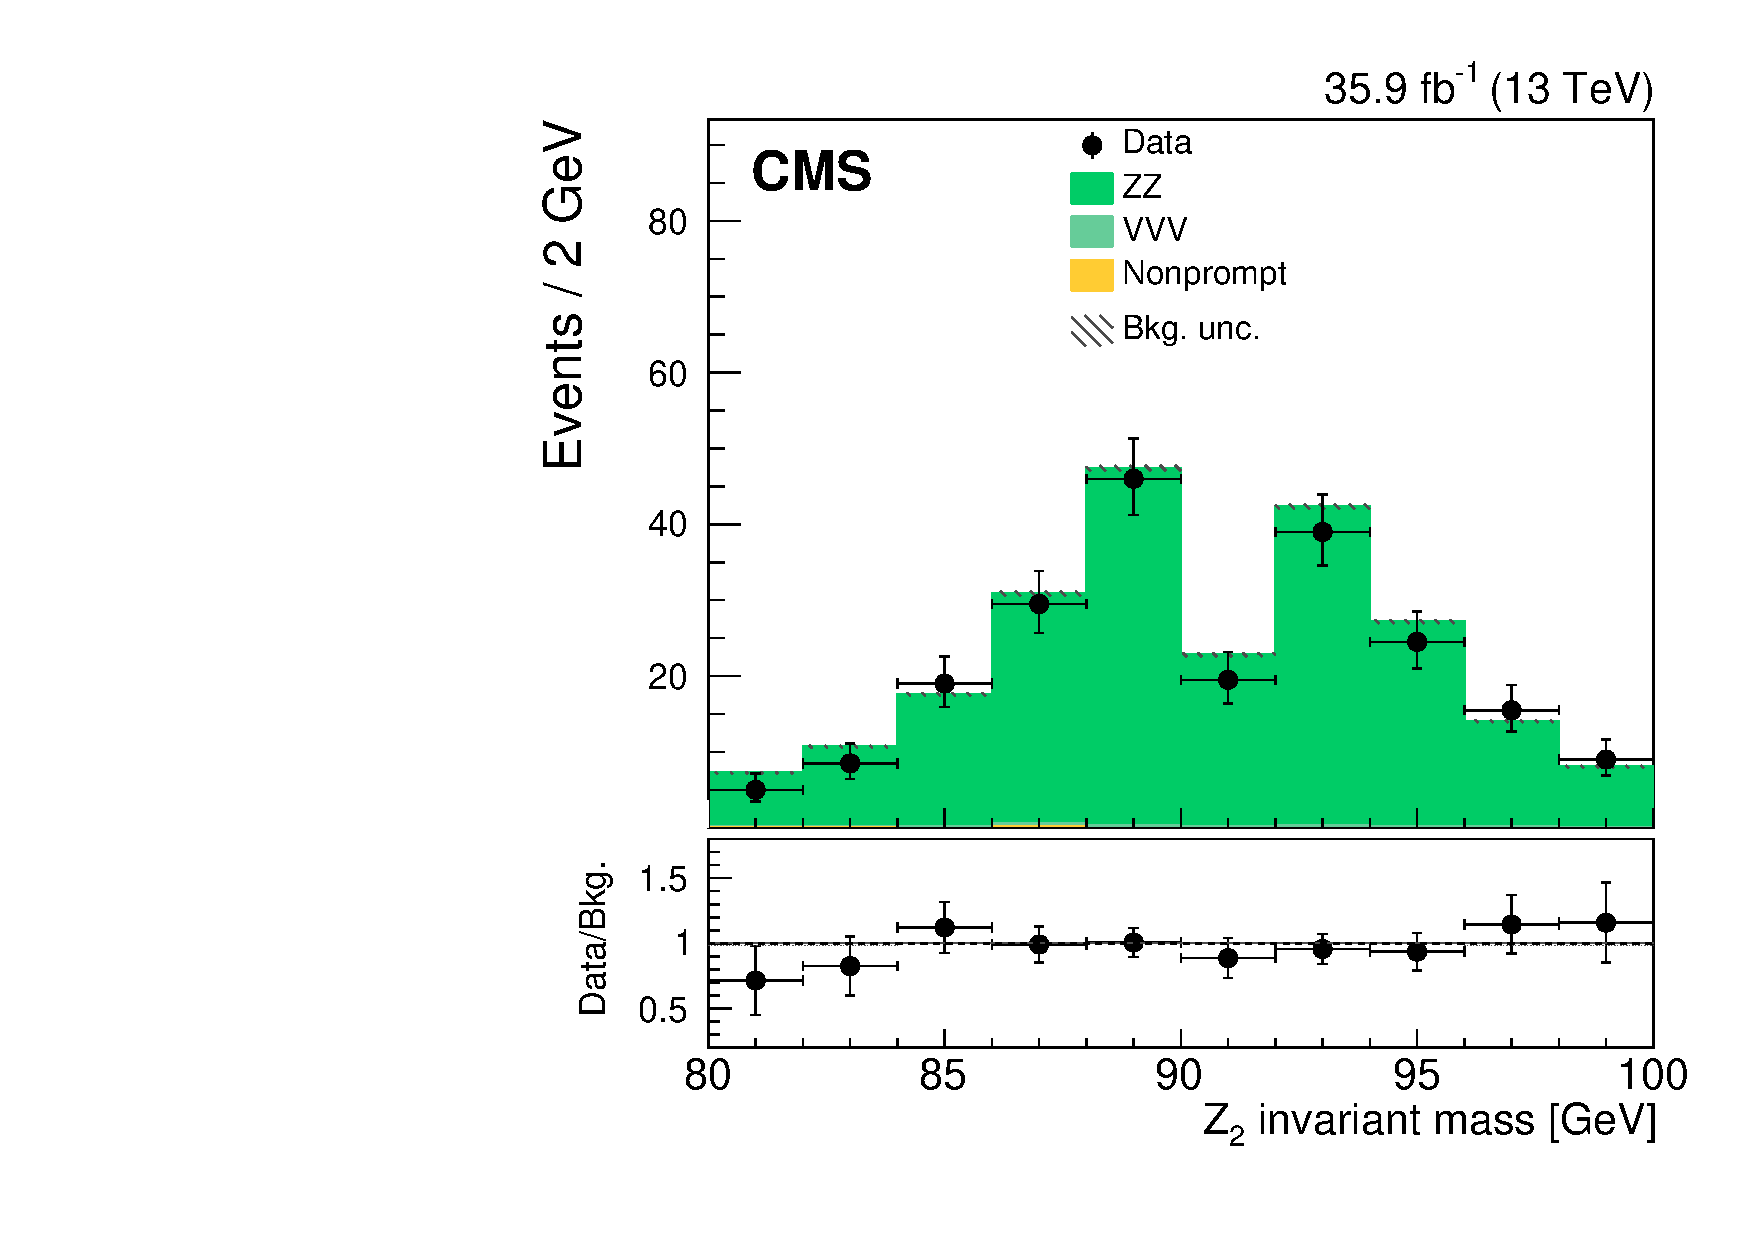
\includegraphics[width=0.48\textwidth]{figures/dibosons/zz4l/mZ2.pdf}
\caption{The invariant masses of the two Z candidates. 
In the right plot, the distribution of $\mathrm{Z}_{2}$ has a cavity close to the Z mass pole because of how $\mathrm{Z}_{1,2}$ are defined.
\label{fig:zz4l_mll}}
\end{figure}

%(..Data):    81.00 +/-   9.00 |   175.00 +/-  13.23 |   224.00 +/-  14.97 |     0.00 +/-   0.00 ->   480.00 +/-  21.91
%(....EM):     0.13 +/-   0.10 |     0.11 +/-   0.10 |     0.66 +/-   0.40 |     0.00 +/-   0.00 ->     0.90 +/-   0.42
%(Zgamma):     0.00 +/-   0.00 |     0.00 +/-   0.00 |     0.00 +/-   0.00 |     0.00 +/-   0.00 ->     0.00 +/-   0.00
%(....WZ):     0.00 +/-   0.00 |     0.00 +/-   0.00 |     0.00 +/-   0.00 |     0.00 +/-   0.00 ->     0.00 +/-   0.00
%( ...ZZ):    77.56 +/-   0.63 |   171.40 +/-   0.96 |   243.01 +/-   1.12 |     0.00 +/-   0.00 ->   491.96 +/-   1.61
%(...VVV):     1.02 +/-   0.12 |     1.94 +/-   0.16 |     2.54 +/-   0.20 |     0.00 +/-   0.00 ->     5.50 +/-   0.28
%(.Higgs):     0.06 +/-   0.18 |     0.41 +/-   0.20 |     0.32 +/-   0.18 |     0.00 +/-   0.00 ->     0.79 +/-   0.32
%(...bkg):    78.77 +/-   0.67 |   173.85 +/-   1.00 |   246.52 +/-   1.22 |     0.00 +/-   0.00 ->   499.15 +/-   1.71
\setlength{\tabcolsep}{12pt}
\begin{table}[!t]
  \caption{Predicted and observed number of events for the ZZ four-lepton selection using $\usedLumi$.
  Only statistical uncertainties are reported.
  \label{tab:zz4lyields}}
  \begin{center}
{\scriptsize
  \begin{tabular}{rllll}
\hline 
Process & $4e$ & $4\mu$ & $2e2\mu$ & Total \\
\hline
ZZ                    &   77.6 $\pm$  0.6 &  171.4 $\pm$  1.0 &  243.0 $\pm$     1.1 &  492.0 $\pm$     1.6 \\ 
VVV                   &    1.0 $\pm$  0.1 &    1.9 $\pm$  0.2 &    2.5 $\pm$     0.2 &    5.5 $\pm$     0.3 \\ 
Nonprompt bkg.        &    0.1 $\pm$  0.1 &    0.1 $\pm$  0.1 &    0.7 $\pm$     0.4 &    0.9 $\pm$     0.4 \\ 
Higgs                 &    0.1 $\pm$  0.1 &    0.4 $\pm$  0.2 &    0.3 $\pm$     0.2 &    0.8 $\pm$     0.3 \\ 
\hline                                                                               
Total                 &   78.7 $\pm$  0.7 &  173.4 $\pm$  1.0 &  246.5 $\pm$     1.2 &  499.2 $\pm$     1.7 \\
\hline                                                                               
Data                  &   81              &  175              &  224                 &  480                 \\
\hline
  \end{tabular}
}
  \end{center}
\end{table}


\begin{figure}[!b]
\centering
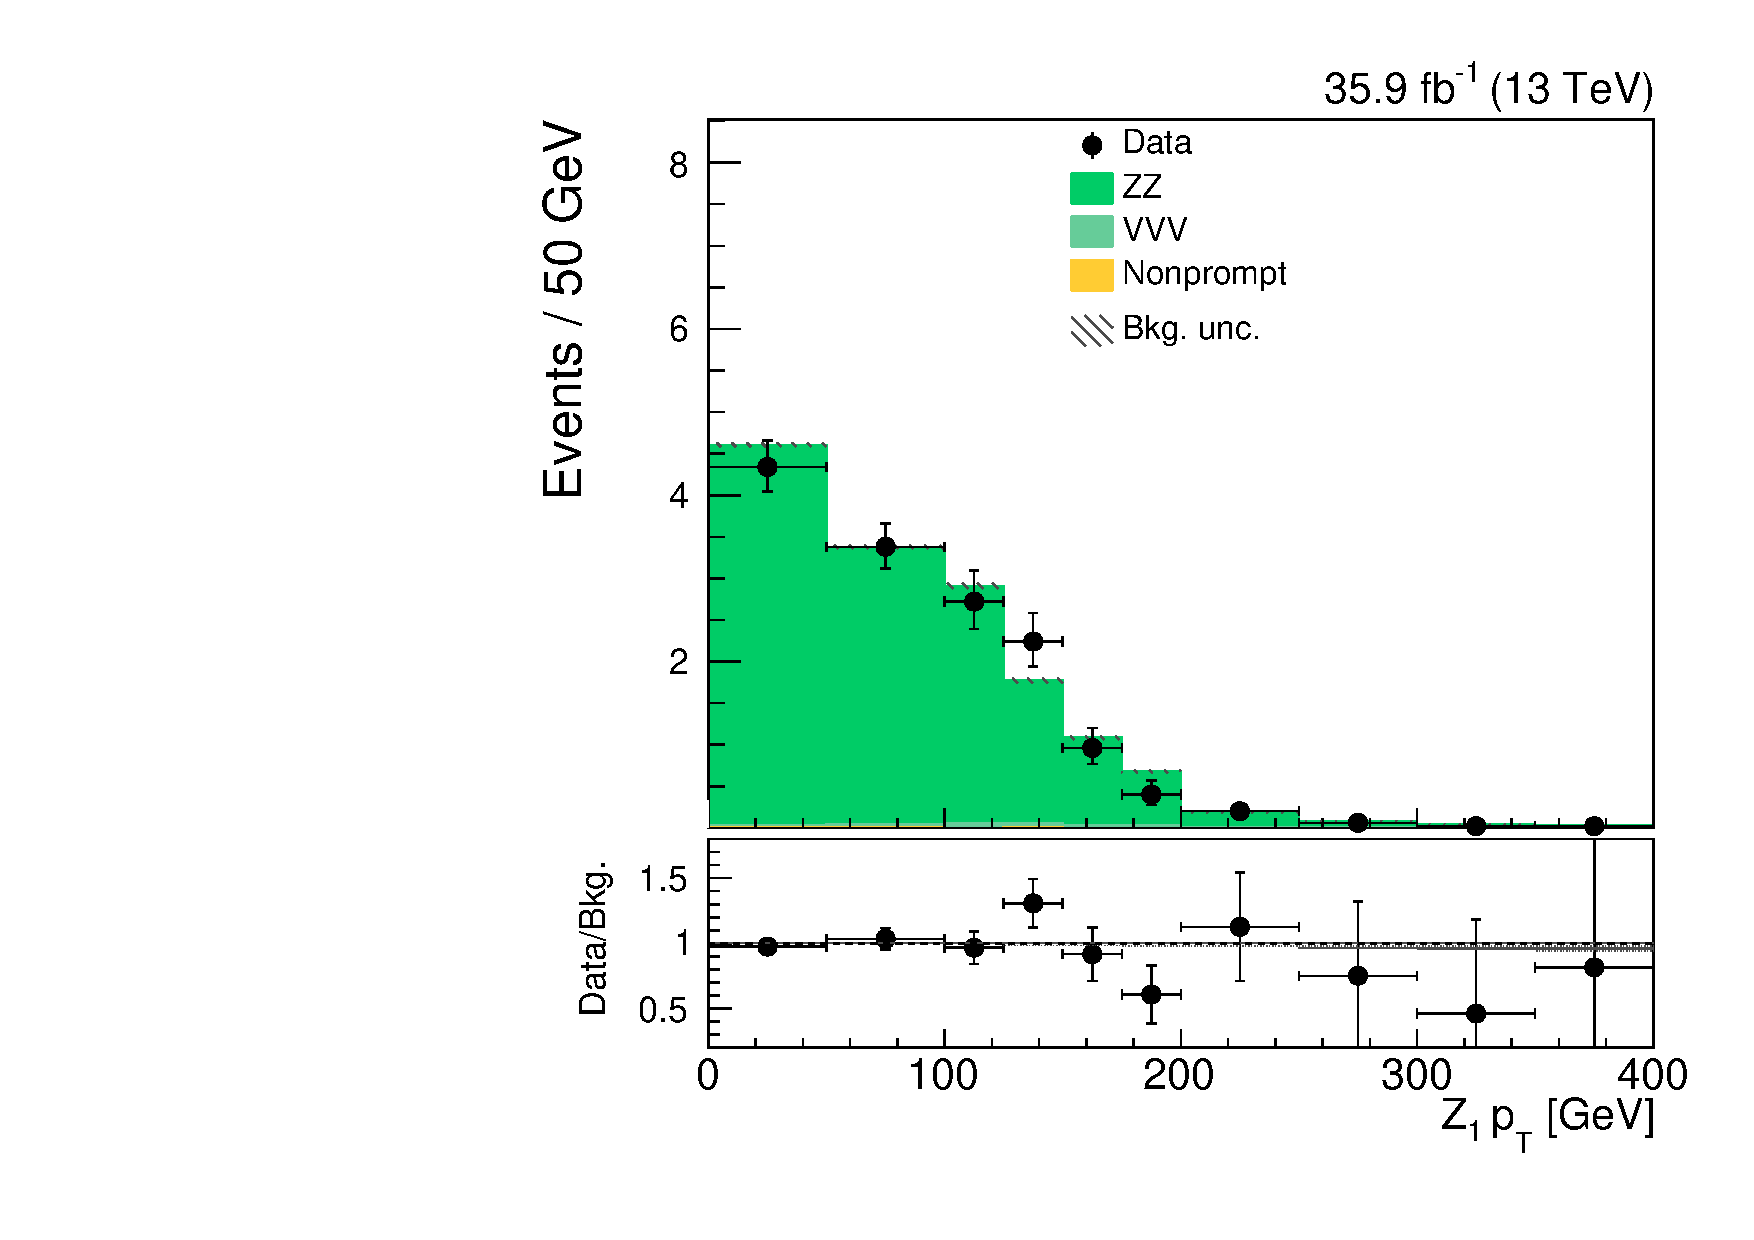
\includegraphics[width=0.48\textwidth]{figures/dibosons/zz4l/pTZ1.pdf}
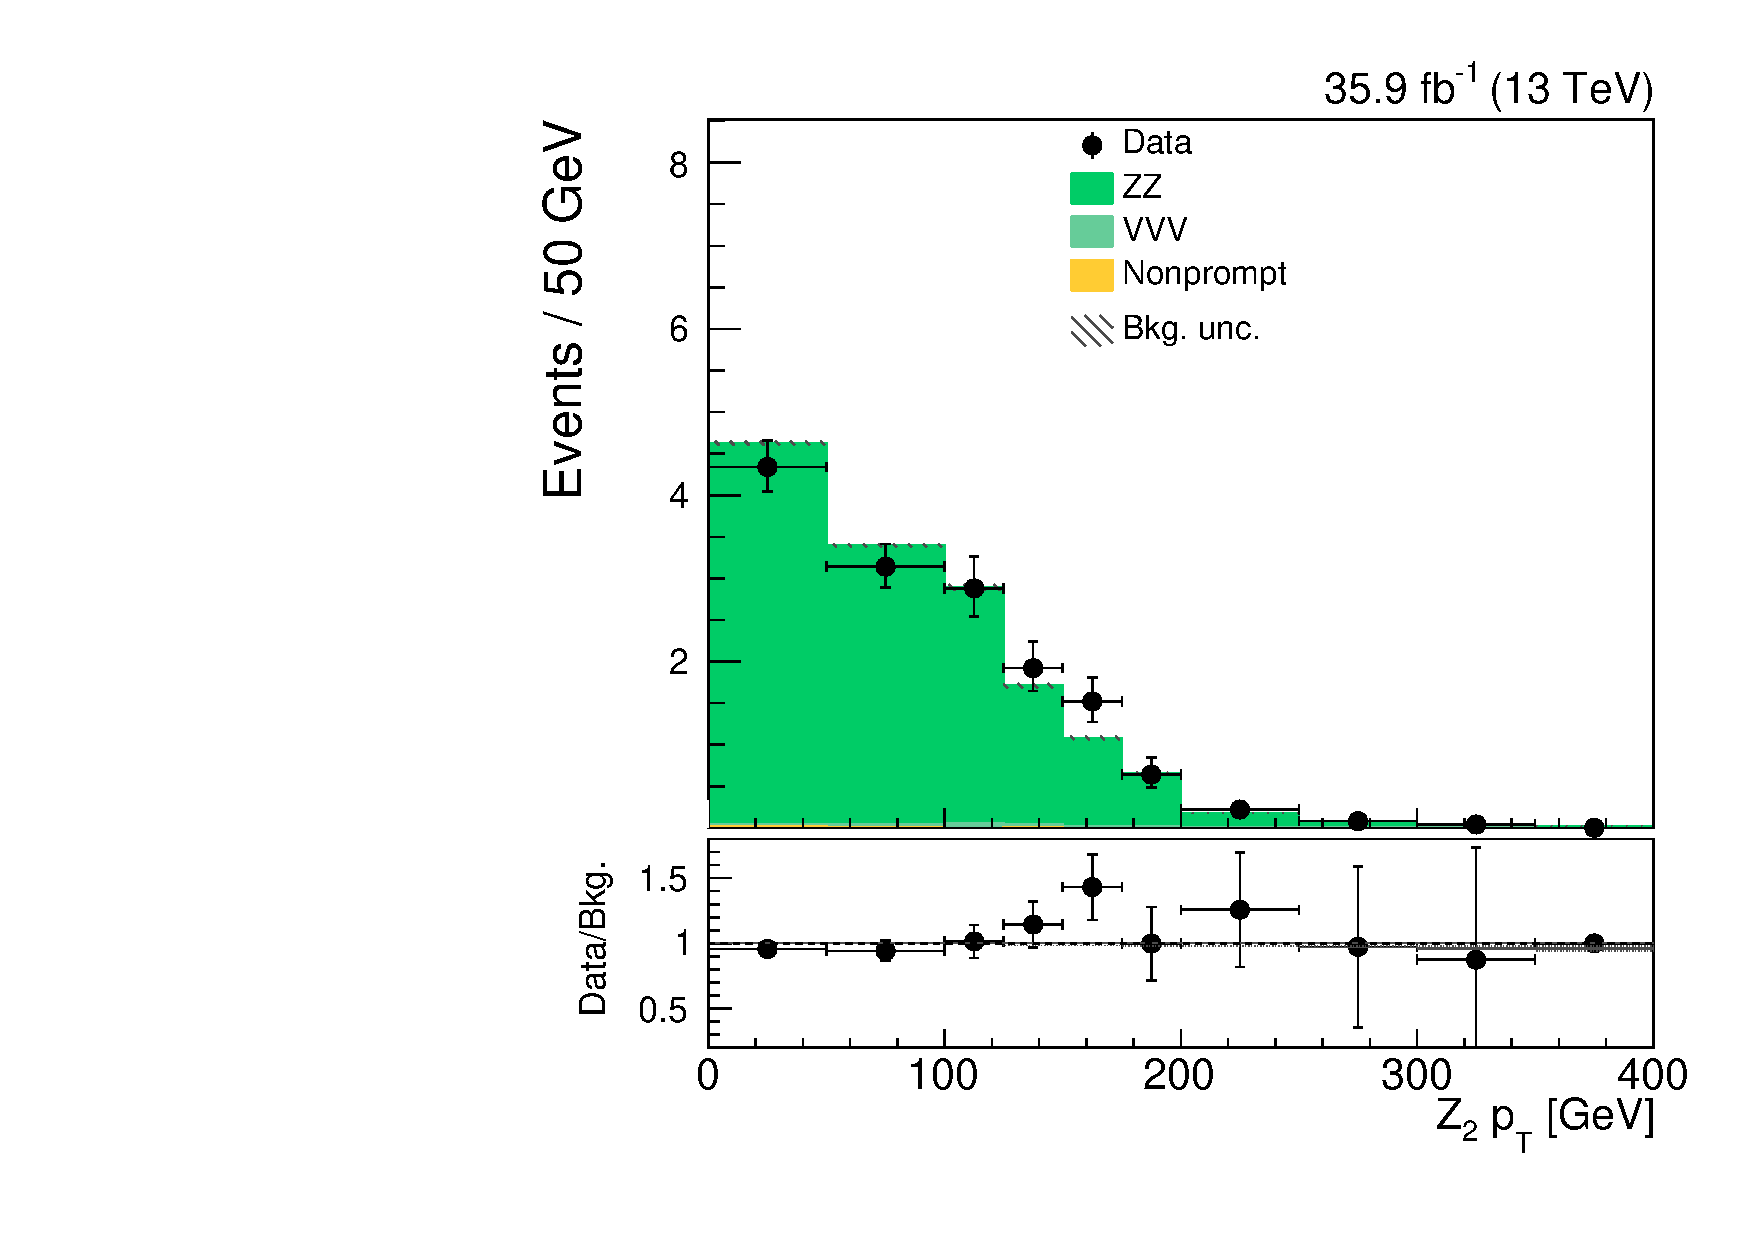
\includegraphics[width=0.48\textwidth]{figures/dibosons/zz4l/pTZ2.pdf}
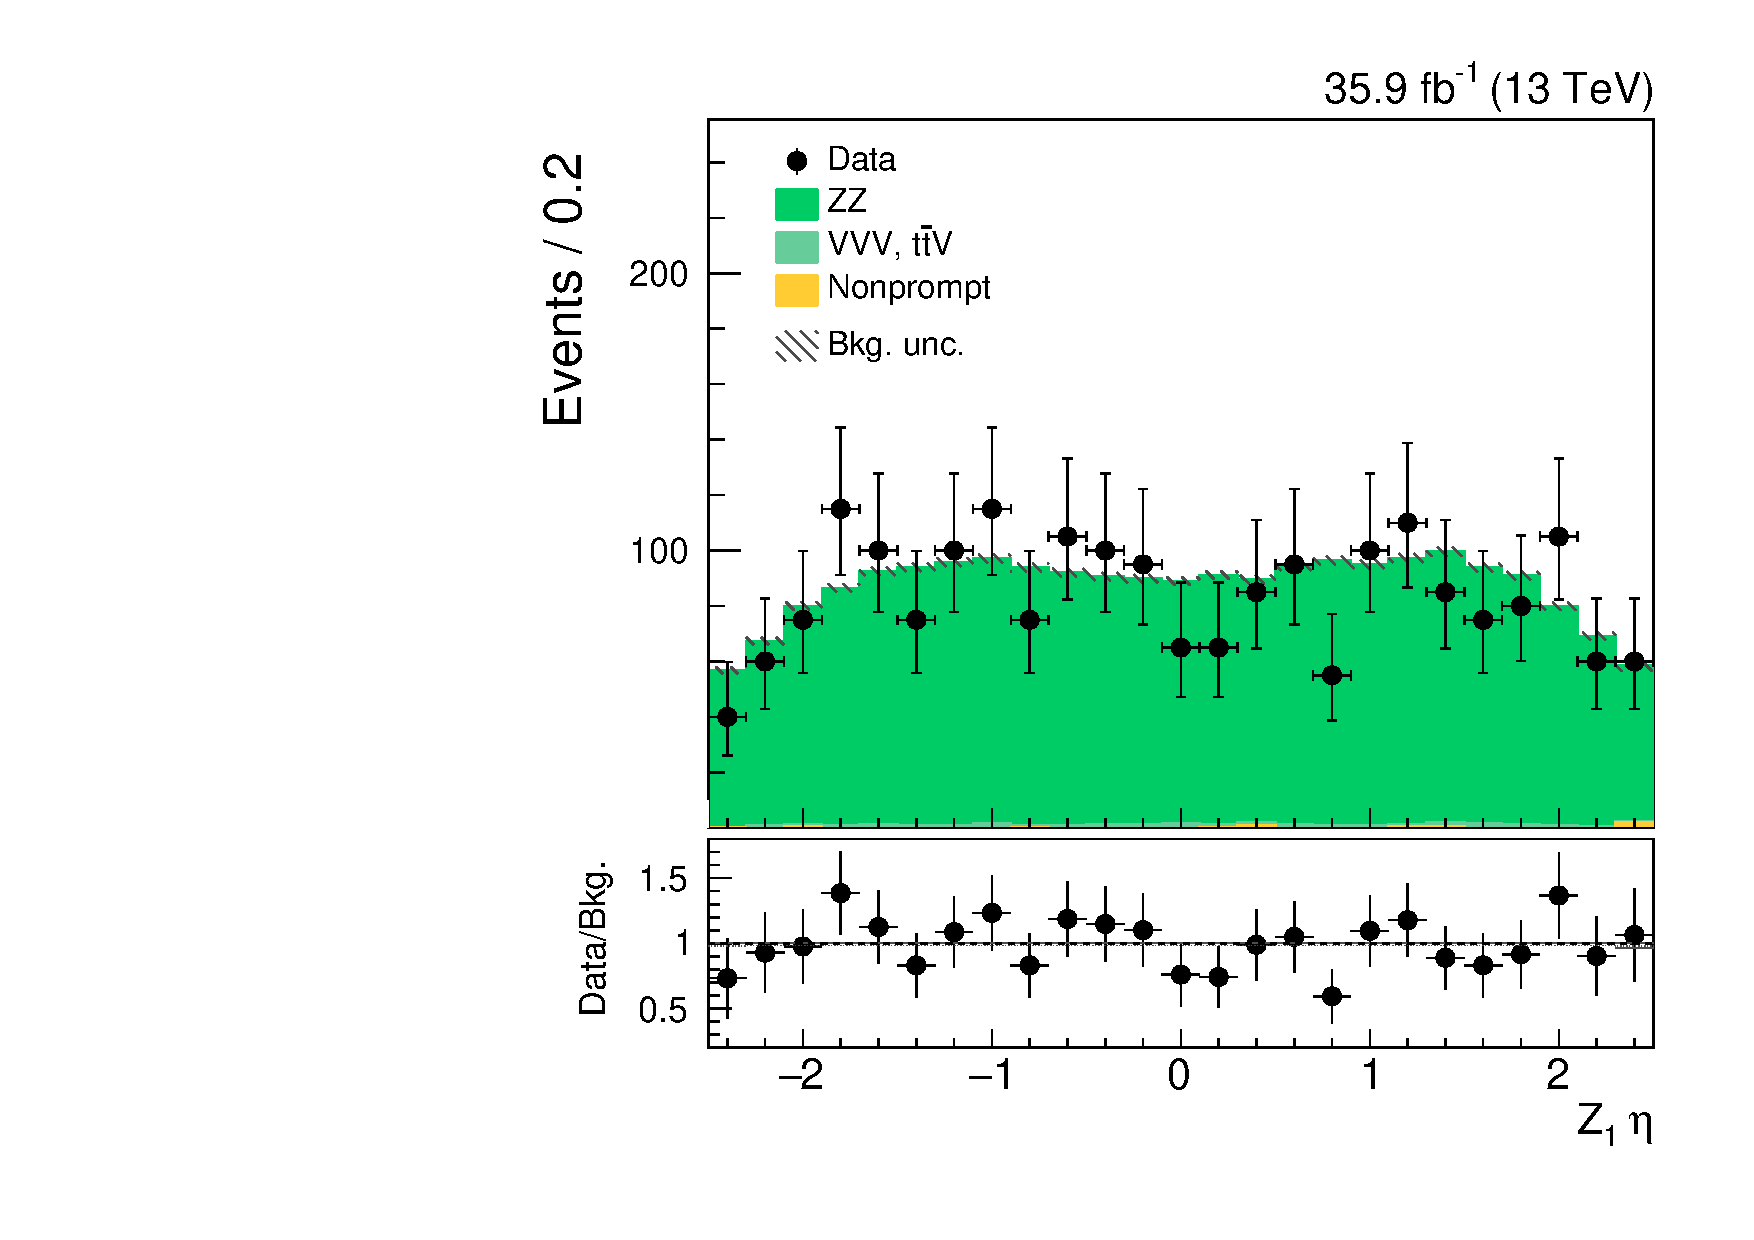
\includegraphics[width=0.48\textwidth]{figures/dibosons/zz4l/etaZ1.pdf}
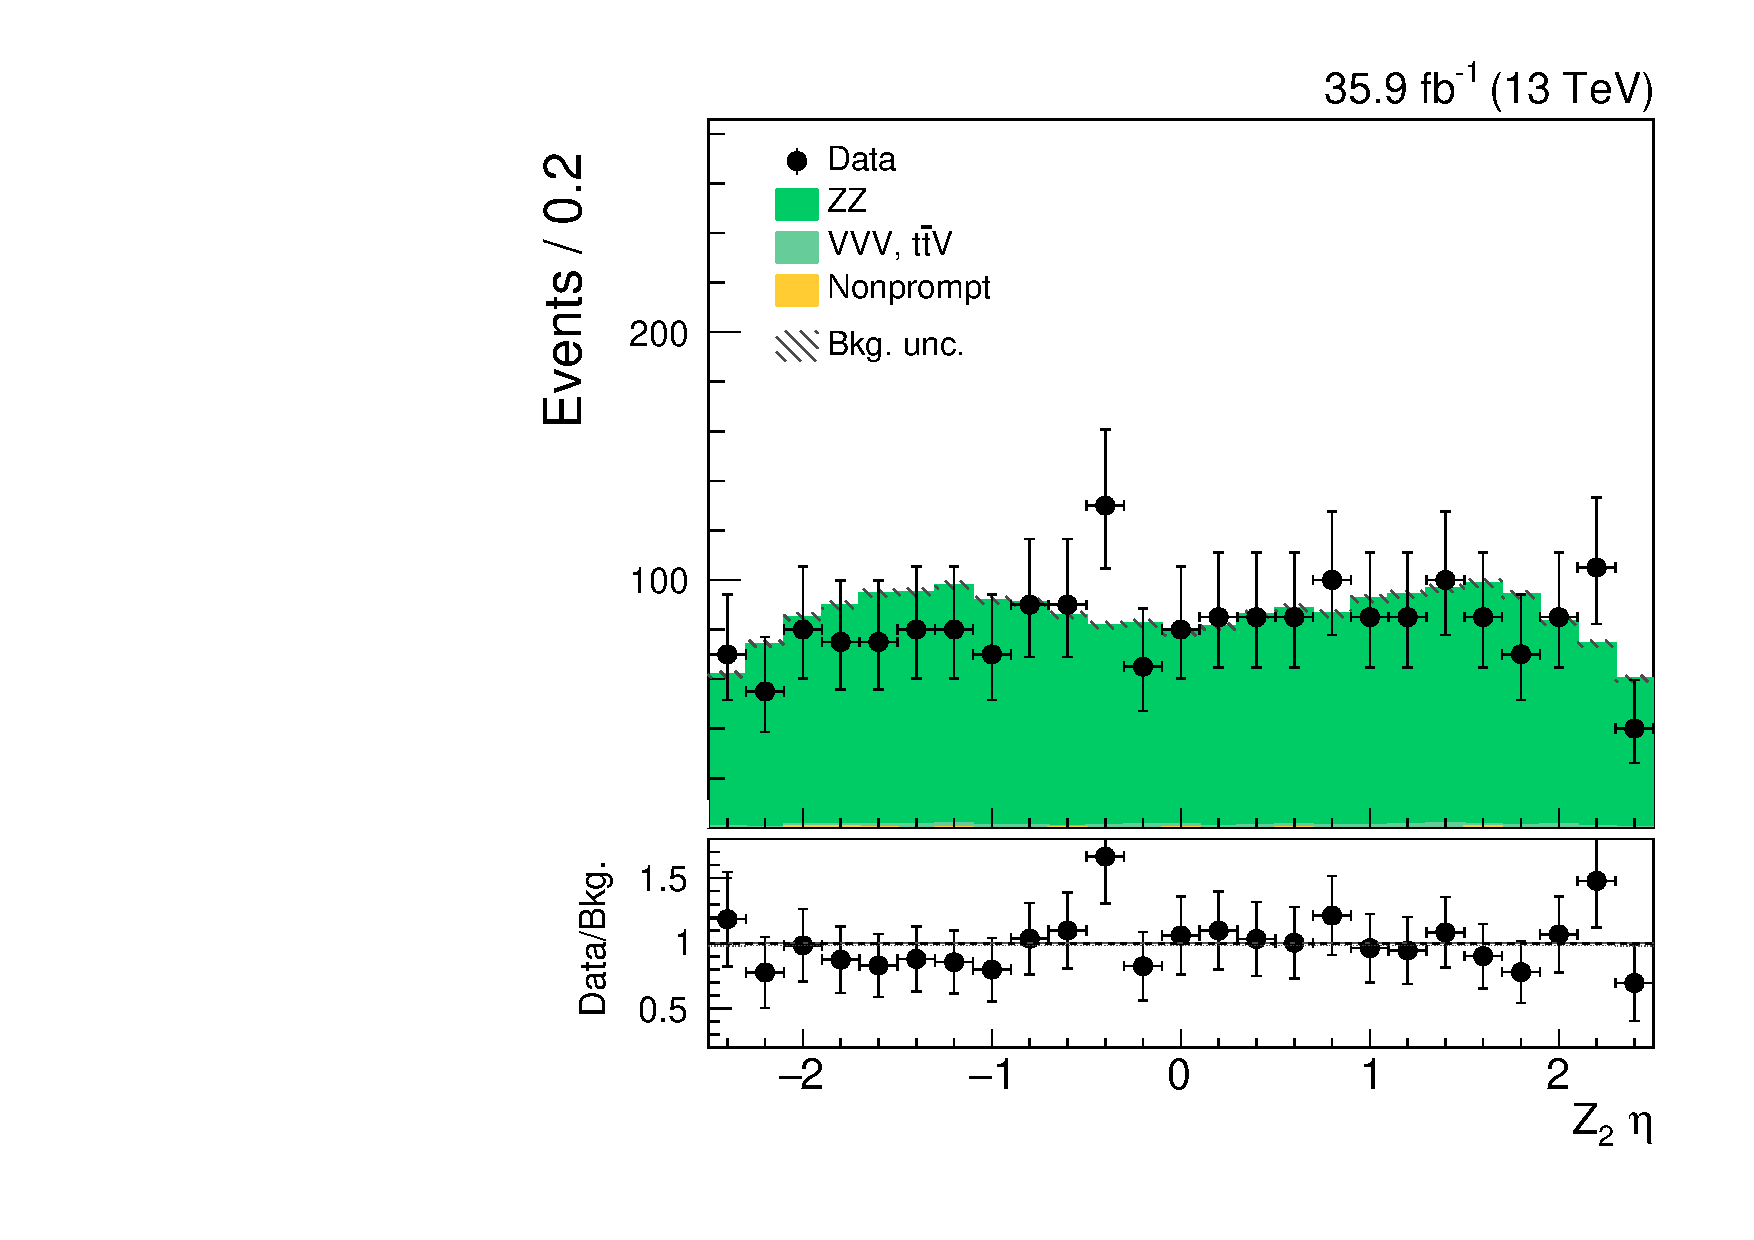
\includegraphics[width=0.48\textwidth]{figures/dibosons/zz4l/etaZ2.pdf}
\caption{Kinematics of the Z candidates. Top: their transverse momenta. Bottom: their pseudorapidities.
\label{fig:zz4l_zpt}}
\end{figure}

\clearpage
\begin{figure}[!h]
\centering
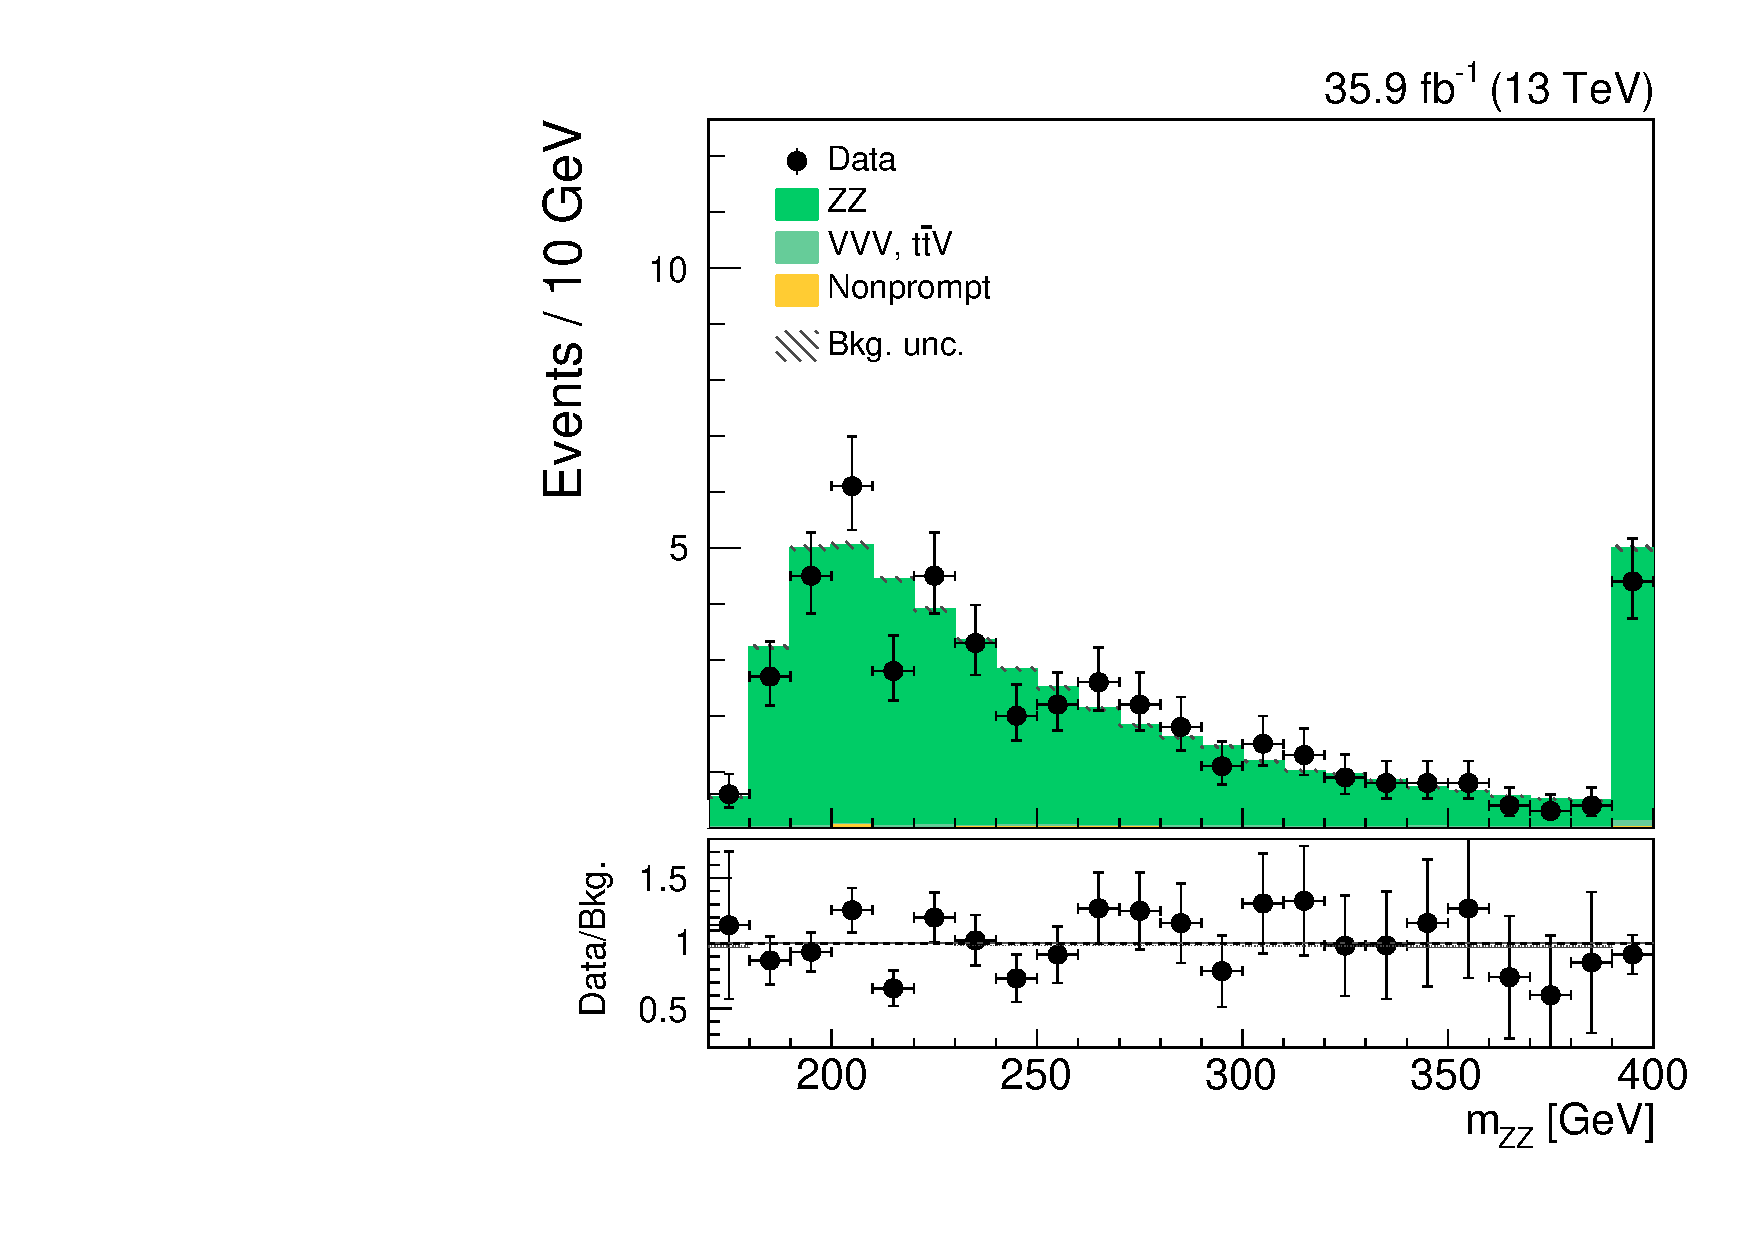
\includegraphics[width=0.48\textwidth]{figures/dibosons/zz4l/mZZ.pdf}
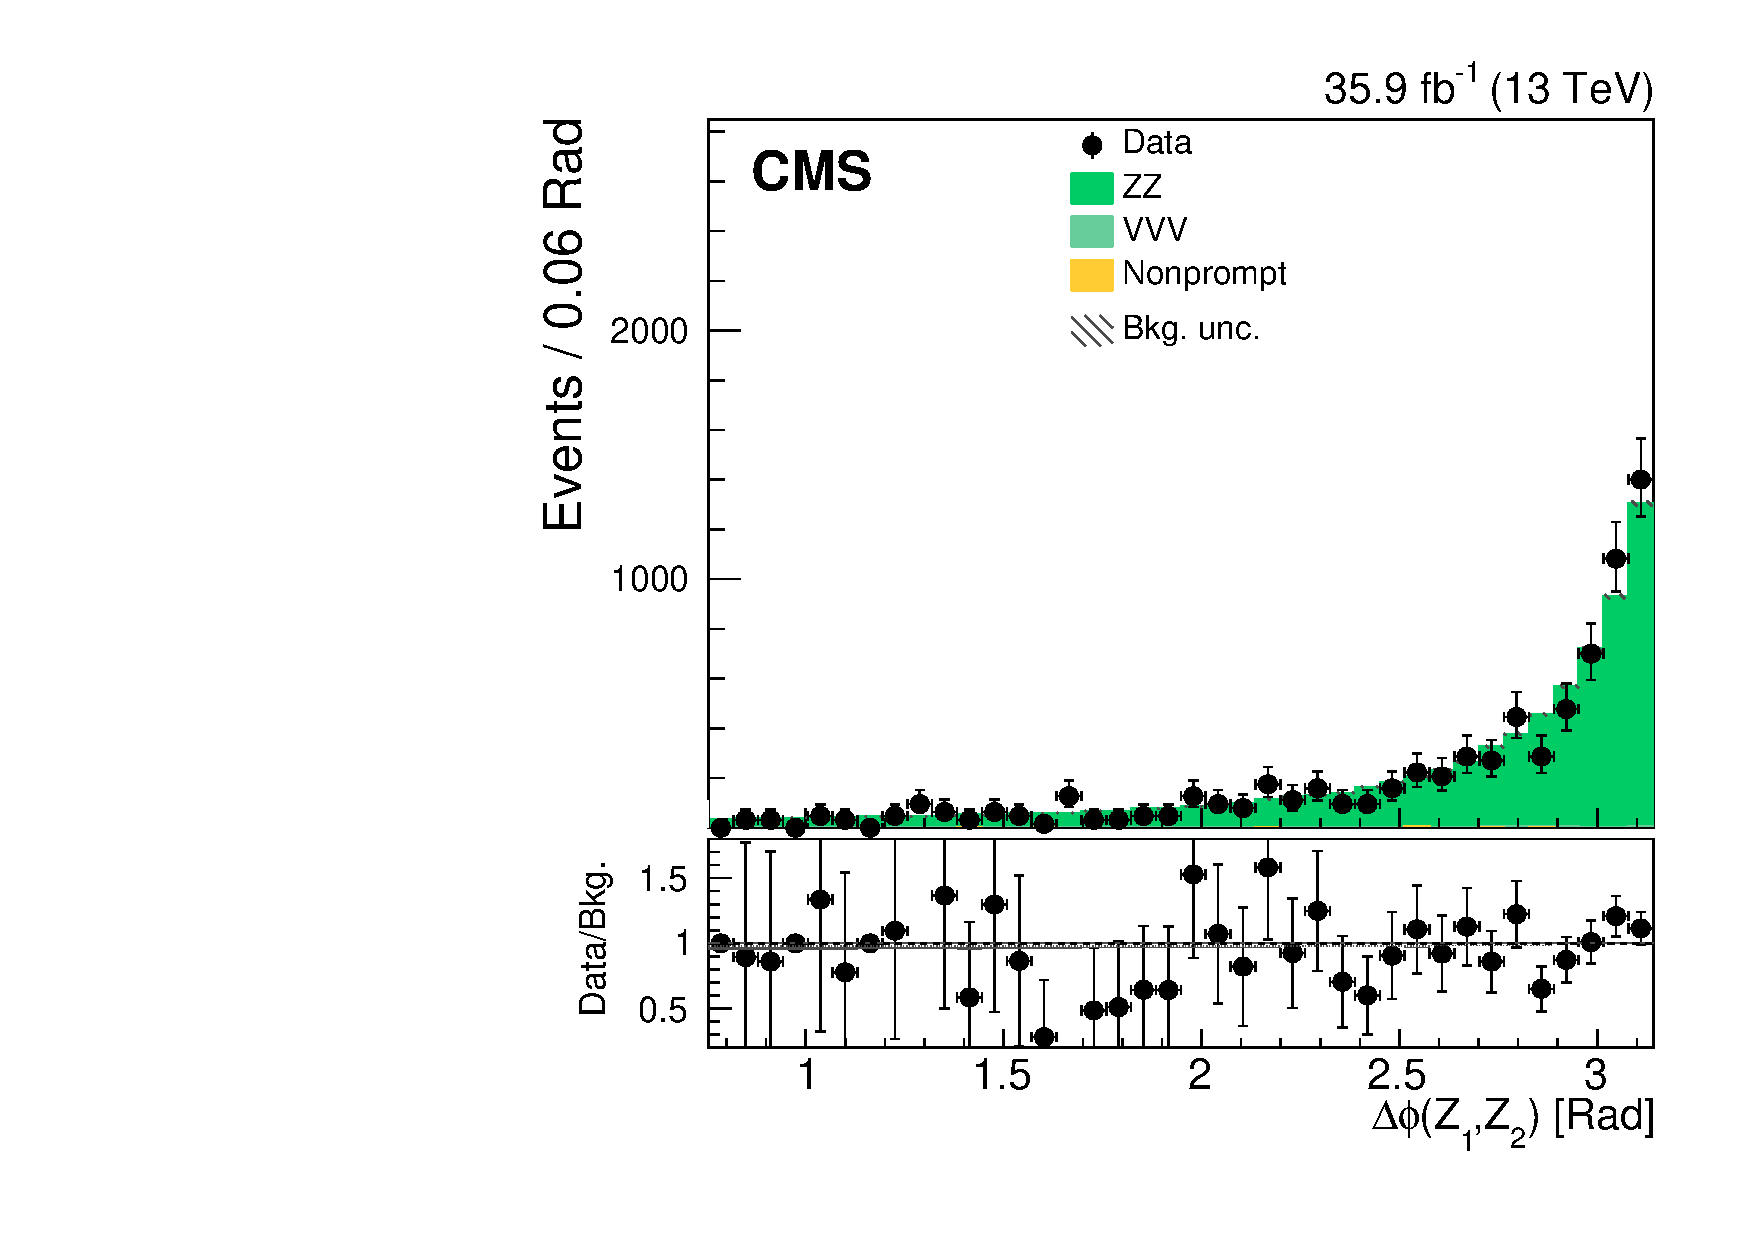
\includegraphics[width=0.48\textwidth]{figures/dibosons/zz4l/dphiZZ.pdf}
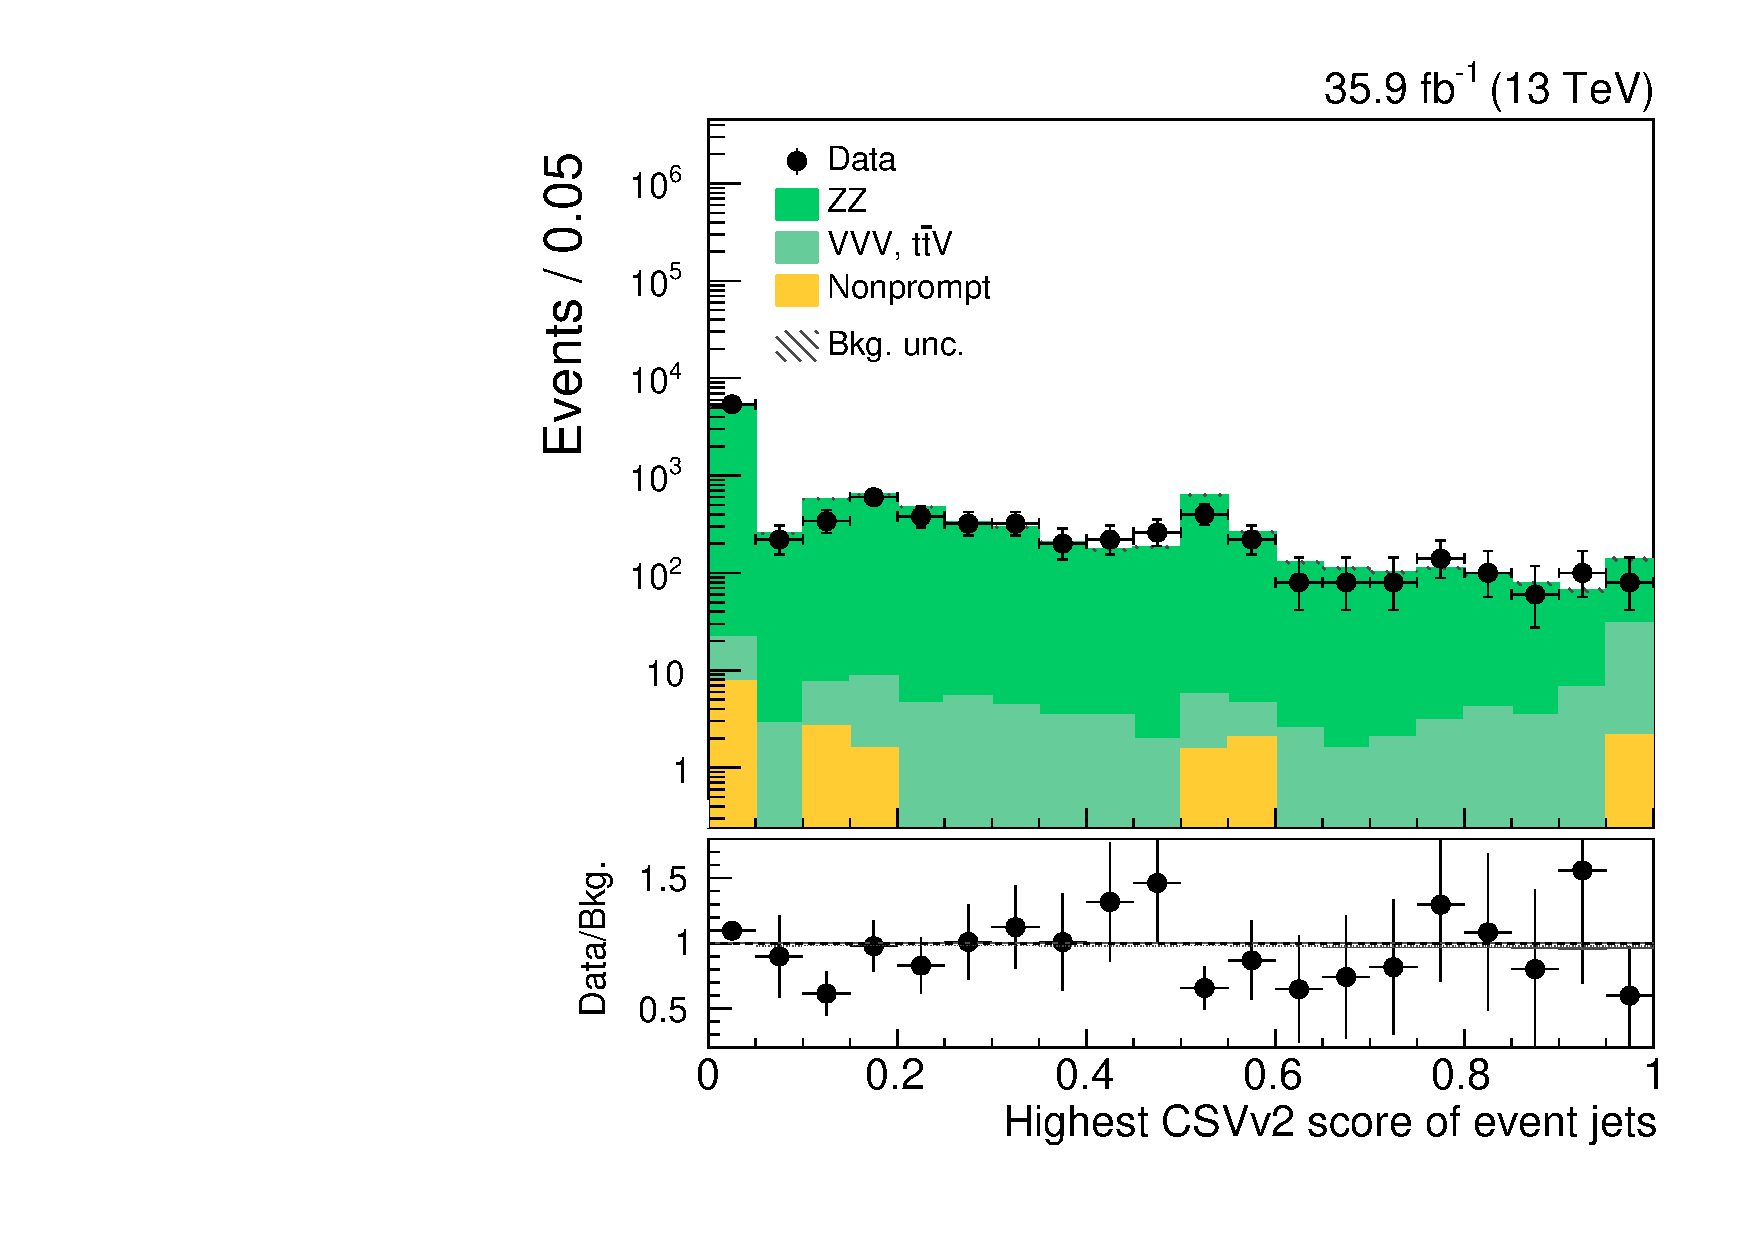
\includegraphics[width=0.48\textwidth]{figures/dibosons/zz4l/bDiscrMax.pdf}
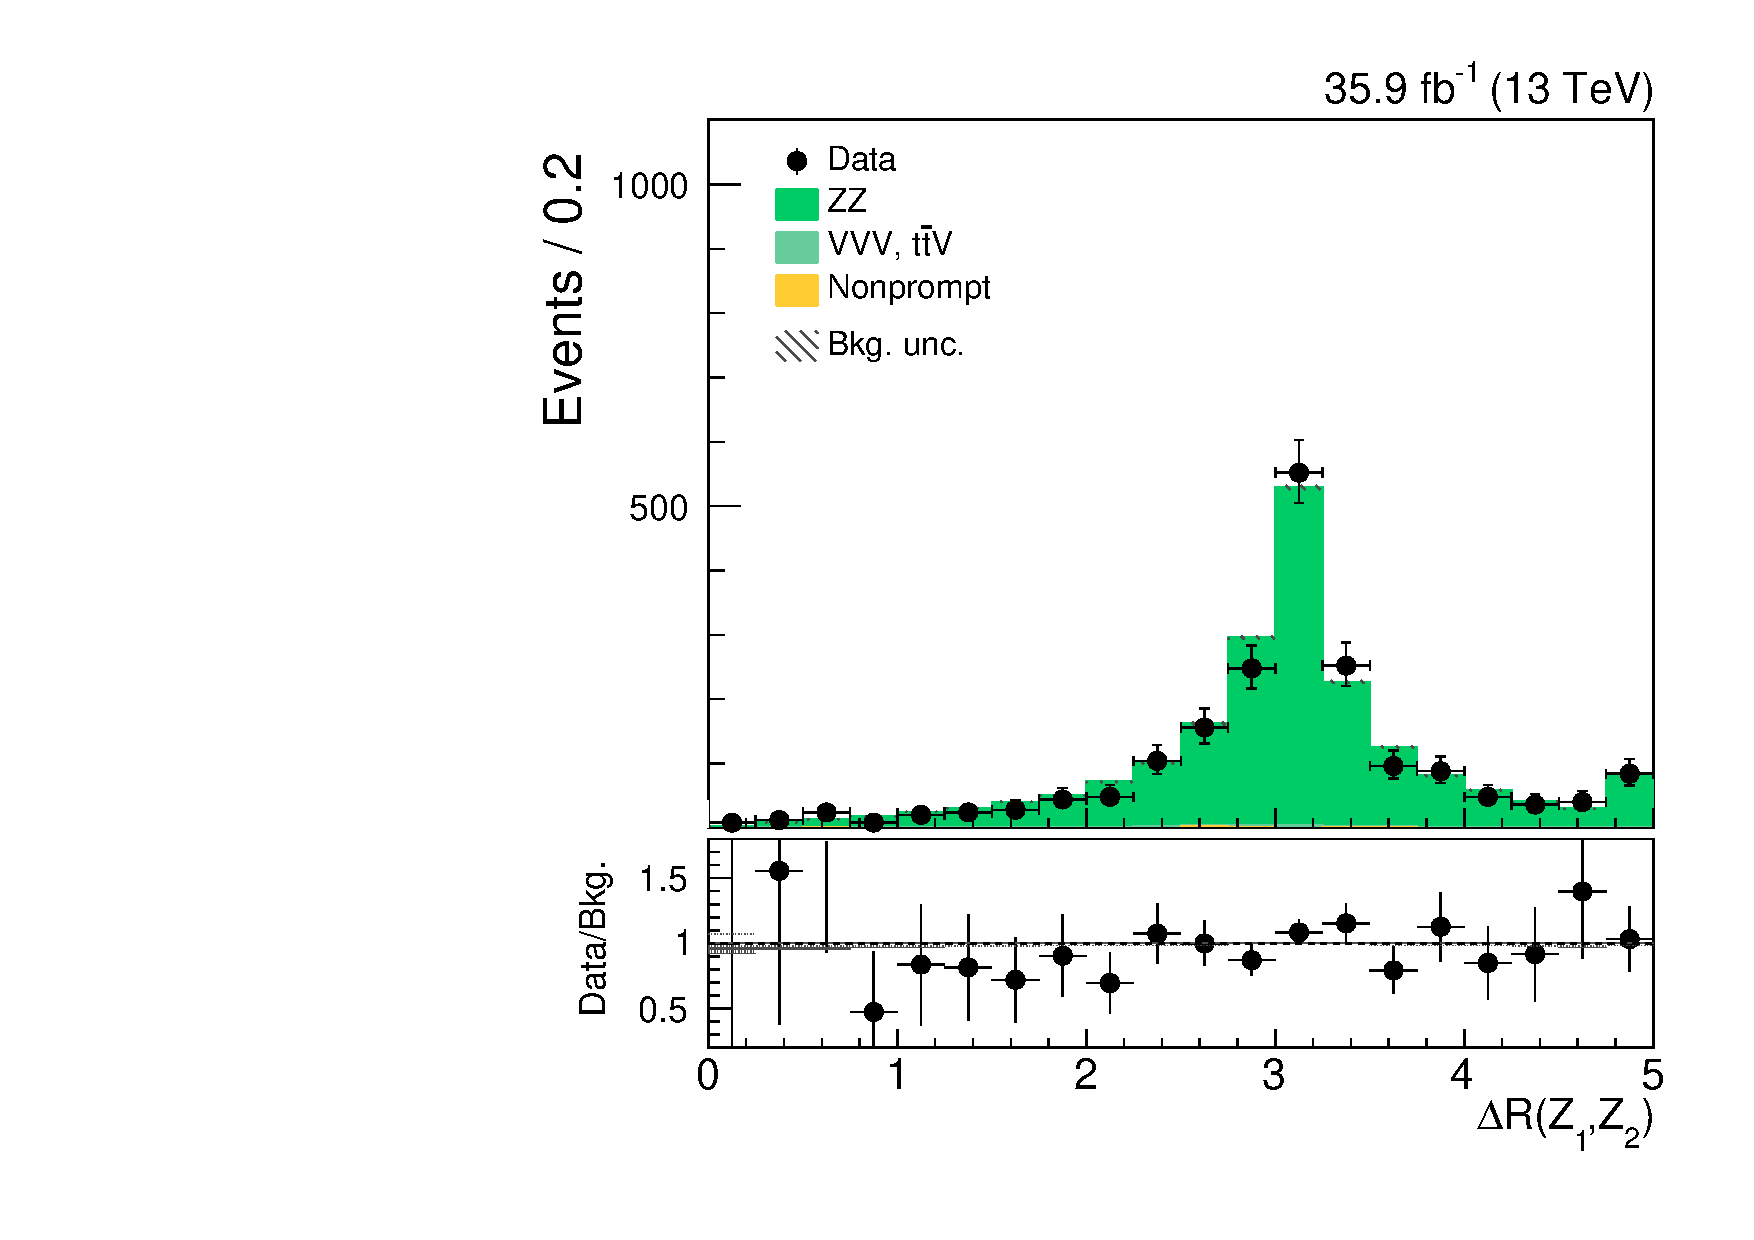
\includegraphics[width=0.48\textwidth]{figures/dibosons/zz4l/dRZ1Z2.pdf}
\caption{More plots of the ZZ data sample.
Clockwise from upper left: diboson invariant mass; azimuthal separation between bosons; the maximum b-tag score of any jet in the event; angular separation between bosons.
The last bin includes the overflow events.
\label{fig:zz4l_moreplots}}
\end{figure}

\section{WZ process}
\label{sec:wz3l}
Next, I will describe how events are selected to observe fully visible WZ production. 
The events must have three well-reconstructed leptons and a nominal amount of $\met$.
A single Z boson candidate is formed from a pair of opposite-charge electrons or muons having invariant mass within 15 \GeV of the Z boson mass.
Additionally, a third well-identified electron or muon is required, representing the W boson.
In the case where there are three electrons or muons,
the Z candidate is chosen unambiguously as the opposite-sign pair whose invariant mass is closest to the Z boson mass.

True WZ events are expected to have an undetectable neutrino in the final state, thus $\met$ of at least 30\GeV is required.
To exclude a region where production of Z bosons with final-state radiation may contribute, the trilepton invariant mass is required to be more than 100 \GeV.
Due to theoretical problems with collinear emission of same-flavor opposite-sign dilepton pairs, the invariant mass of any opposite-sign lepton pair ($m_{2\Lep}$) is required to be larger than $4\GeV$.
These requirements follow precedent for the measurement of the $\WZ$ production cross section with CMS~\cite{Khachatryan:2016tgp}.

Since there is no danger of contamination, no veto on additional hadronically-decaying $\tau$ leptons is applied.
A relaxed b-jet veto is applied which rejects events where a jet passes the most stringent b-jet identification requirement.
This, along with the Z candidate invariant mass requirement, is useful for rejecting ditop background.

The selection yields in simulation and data for the WZ analysis are shown in Table~\ref{tab:wz3lyields}.
Kinematic variables of the bosons, and variables used in the selection, are shown in Figures~\ref{fig:wz3l_z},~\ref{fig:wz3l_purity}, and~\ref{fig:wz3l_w}.
In particular, note the presence of the expected Jacobian peak in the W boson transverse mass distribution in Figure~\ref{fig:wz3l_w}.
The transverse mass is calculated in the transverse $(r,\phi)$ plane using the 
third lepton ($\vec{\mathbf{p}}_\mathrm{T}^\ell$) and missing energy ($\vec{\mathbf{p}}_\mathrm{T}^\mathrm{miss}$) vectors:
\begin{equation}
\label{eq:mt}
\begin{split}
m_\mathrm{T} & = \sqrt{m_\ell^2 + m_\nu^2 + 2(E_\ell E_\nu -\vec{\mathbf{p}}_\mathrm{T}^\ell \cdot \vec{\mathbf{p}}_\mathrm{T}^\mathrm{miss})} \\ 
& \approx \sqrt{2\:|\vec{\mathbf{p}}_\mathrm{T}^\ell|\:|\vec{\mathbf{p}}_\mathrm{T}^\mathrm{miss}|\:(1 - \mathrm{cos}\:\Delta\phi)} \qquad \mathrm{for}\:m_\ell,\:m_\nu\approx0
\end{split}
\end{equation}
where $\Delta\phi$ is the azimuthal separation between those vectors.

\begin{figure}[!bh]
\centering
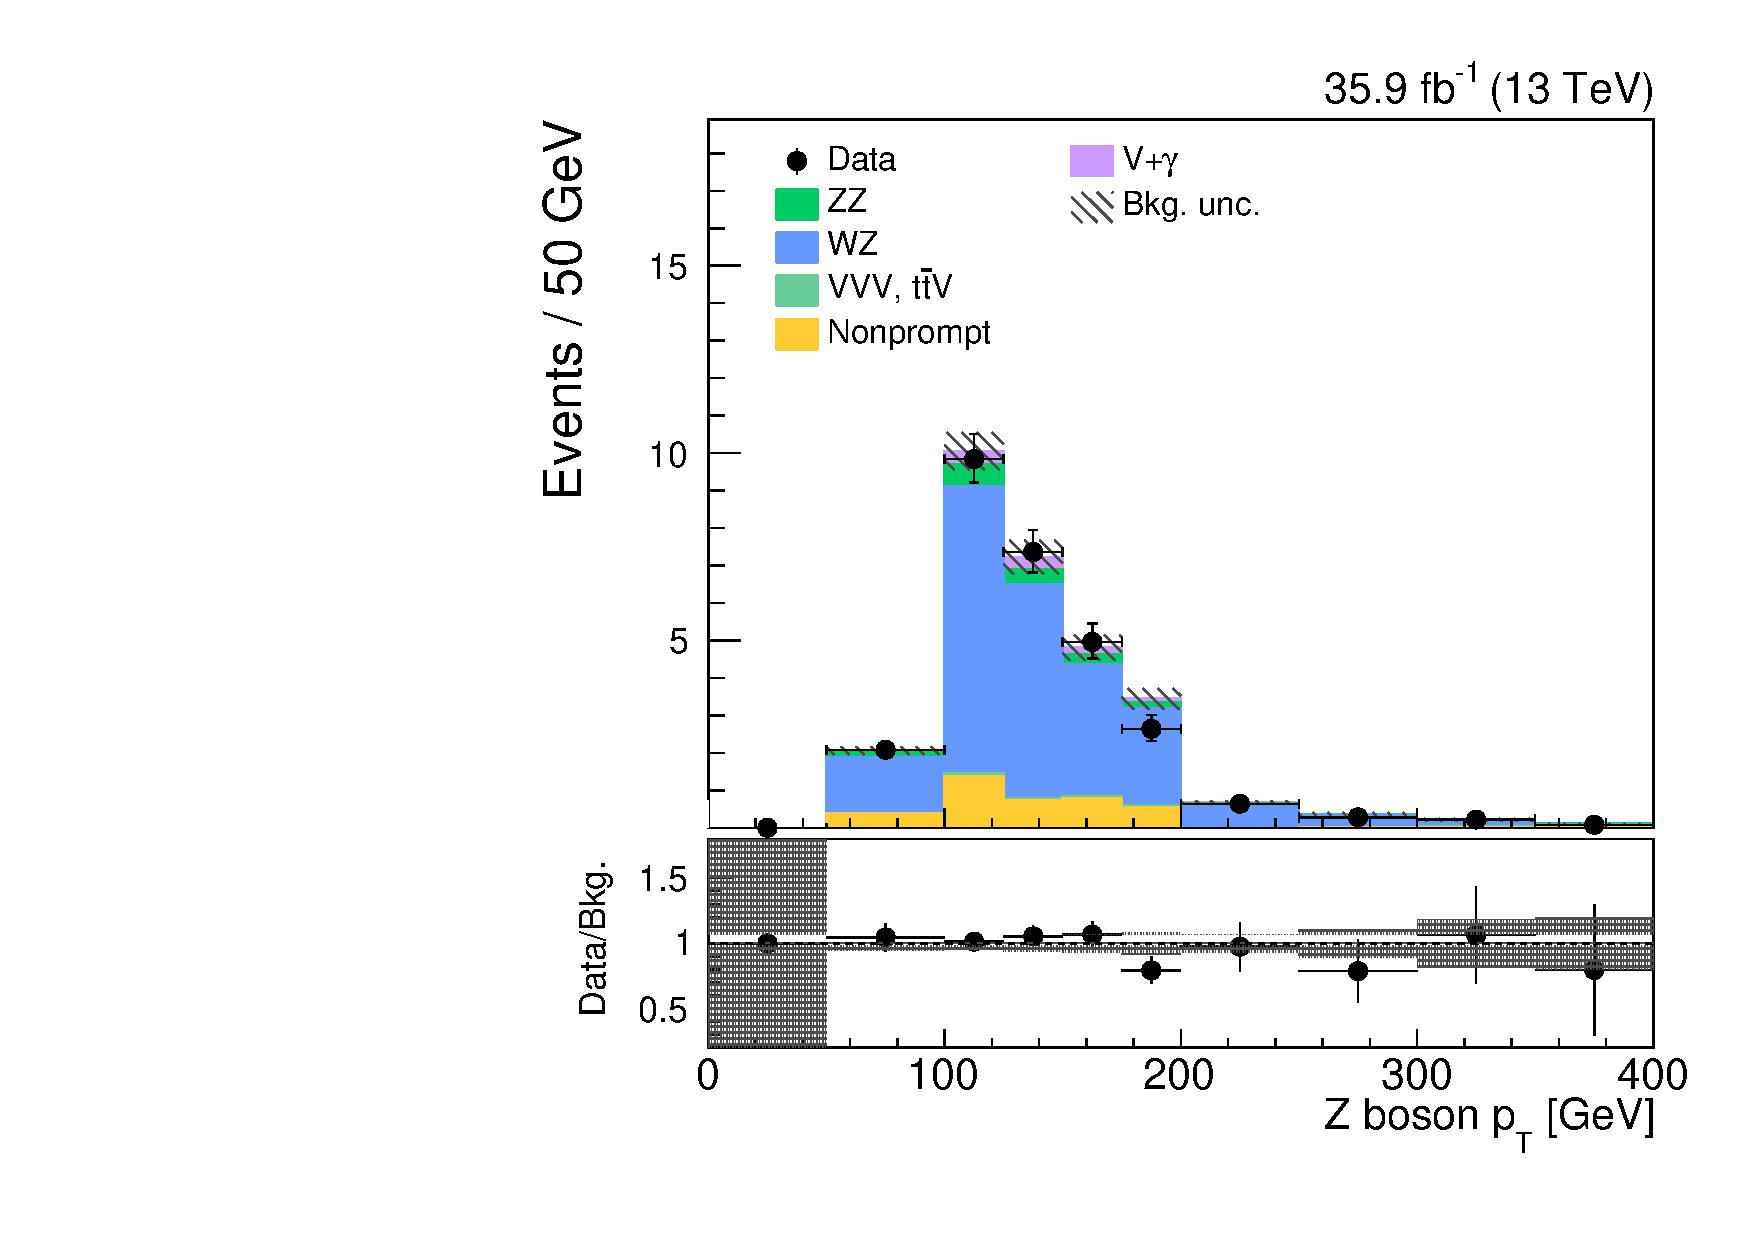
\includegraphics[width=0.48\textwidth]{figures/dibosons/wz3l/pTZ.pdf}
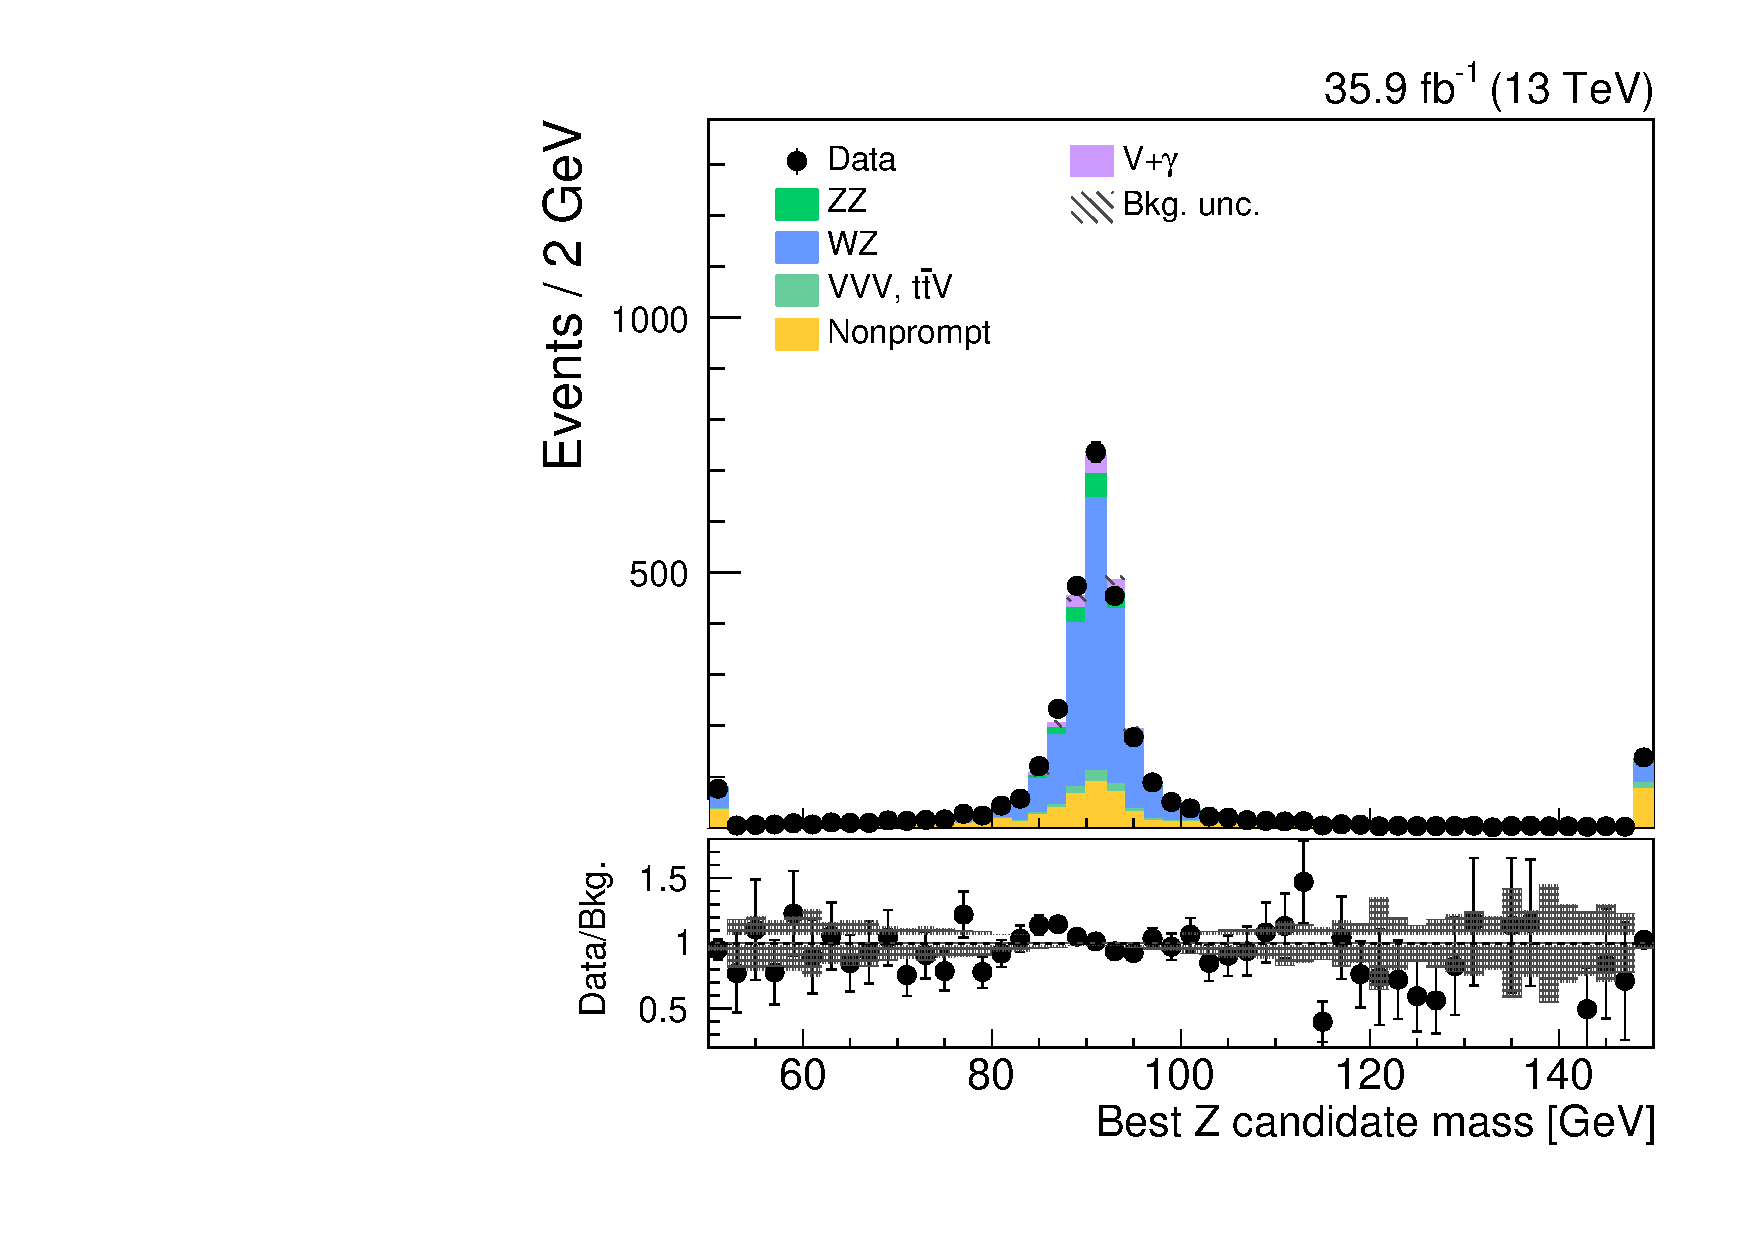
\includegraphics[width=0.48\textwidth]{figures/dibosons/wz3l/minMassZ_Nminus1.pdf}
\caption{The transverse momentum and invariant mass of the reconstructed Z boson candidate.
The last bin includes the overflow events.
\label{fig:wz3l_z}}
\end{figure}
\clearpage

\begin{figure}[!t]
\centering
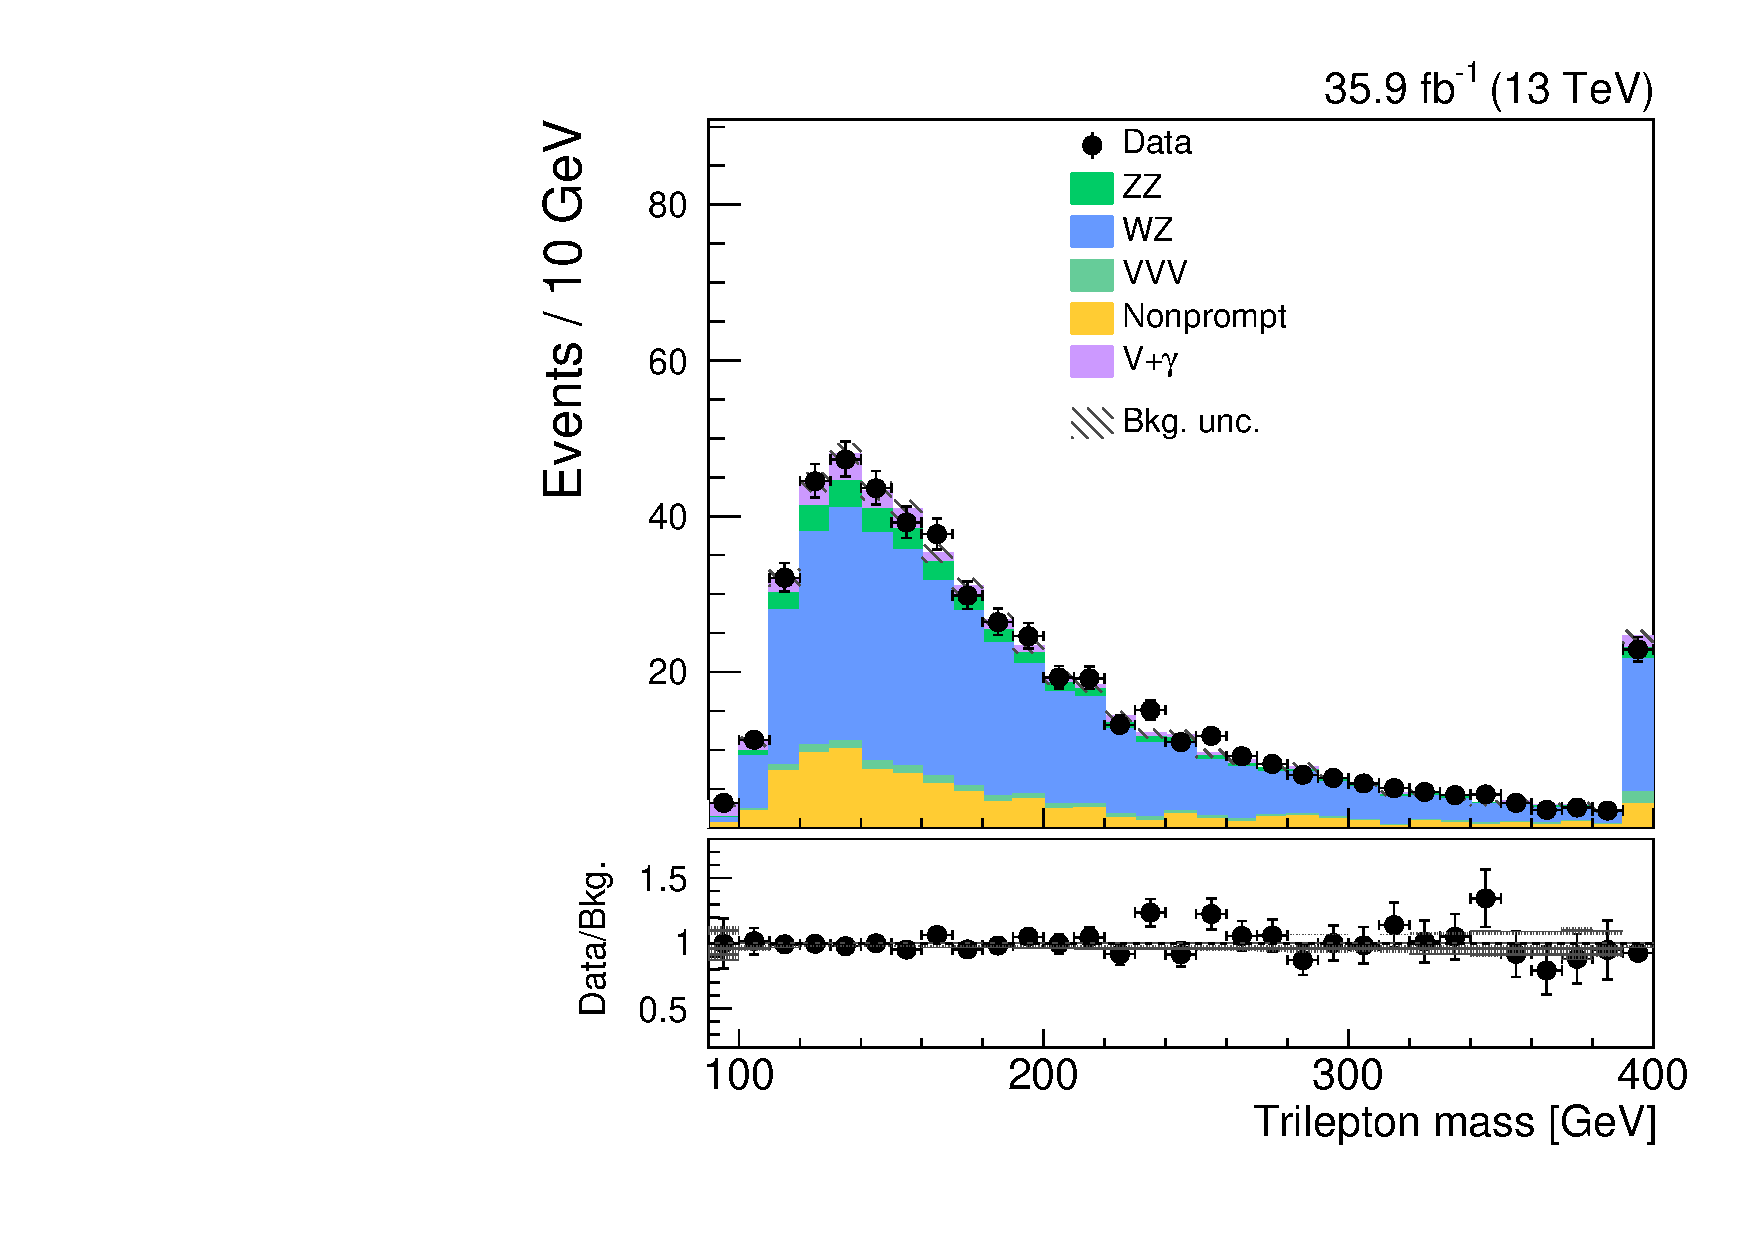
\includegraphics[width=0.48\textwidth]{figures/dibosons/wz3l/m3l_Nminus1.pdf}
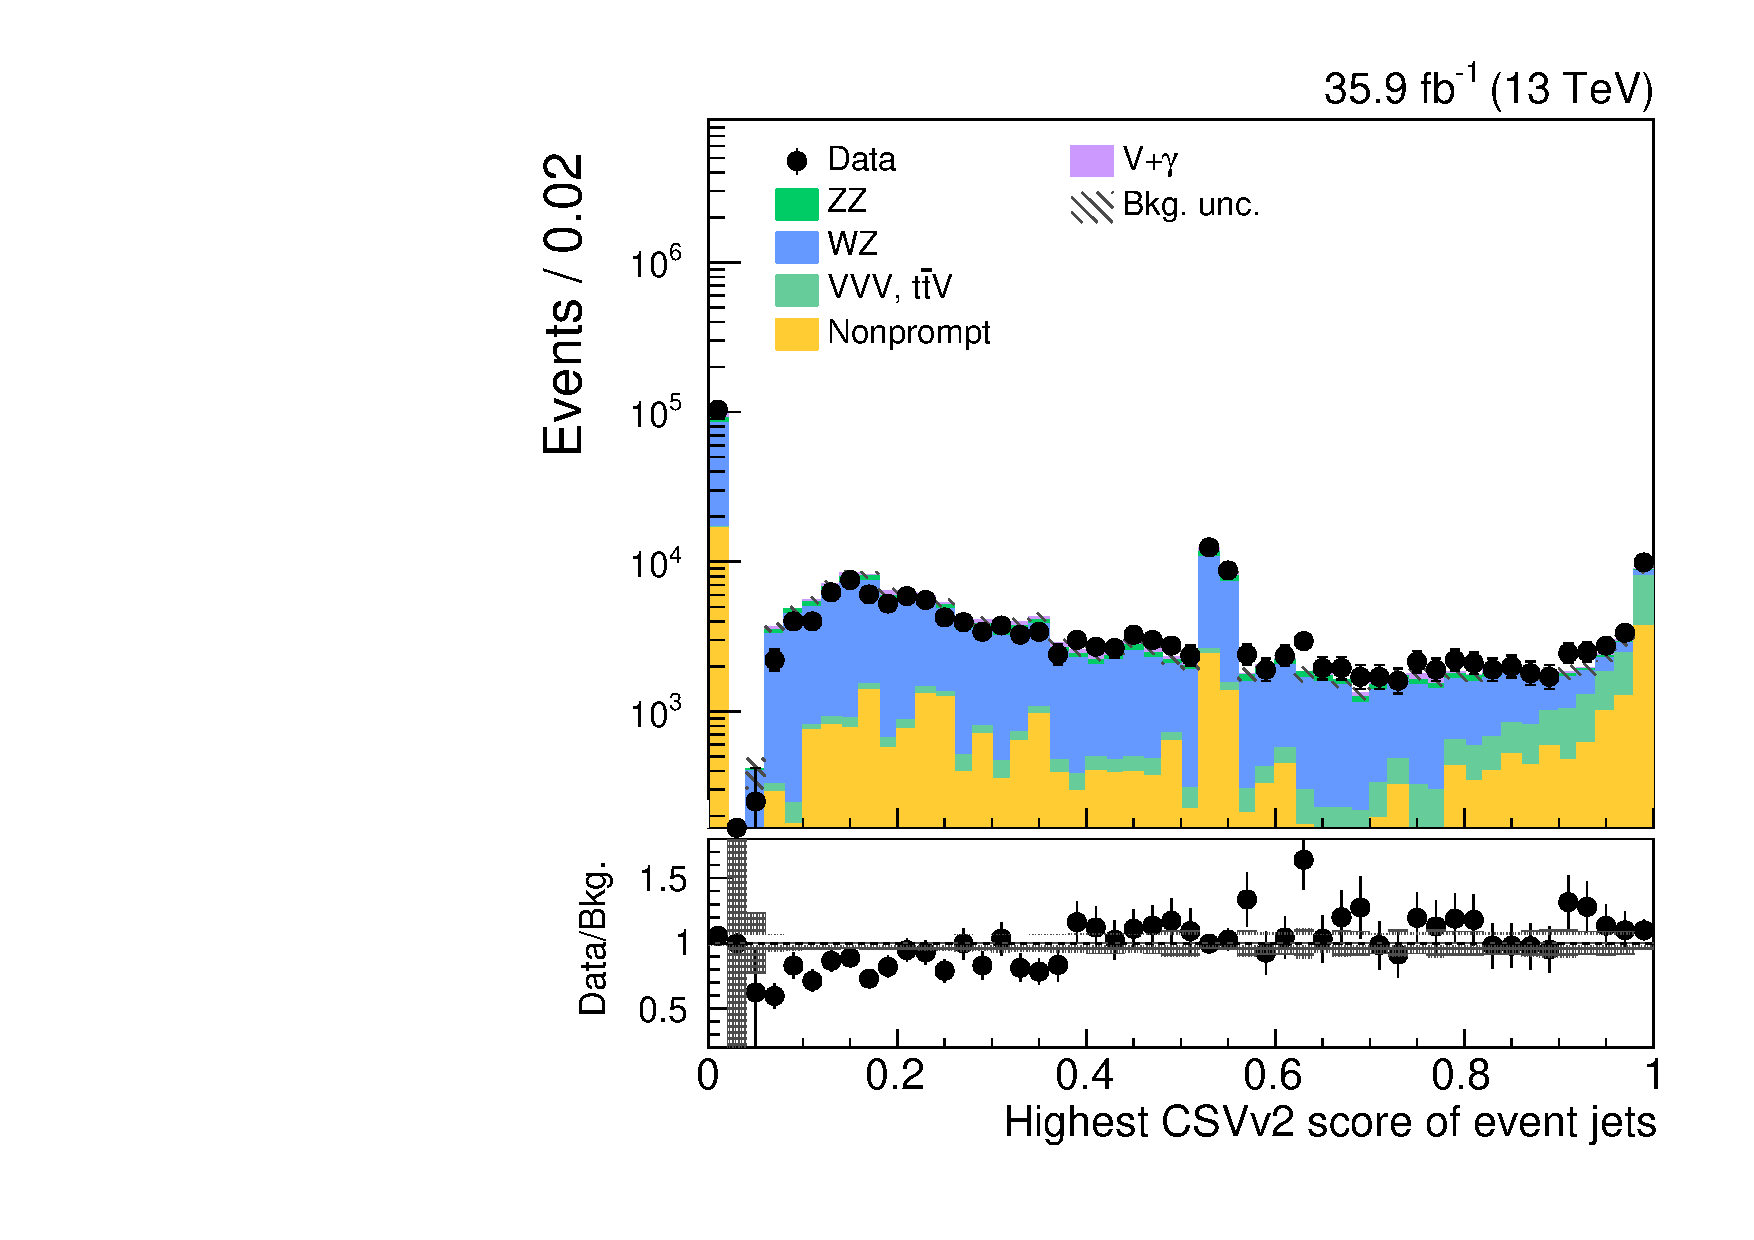
\includegraphics[width=0.48\textwidth]{figures/dibosons/wz3l/bDiscrMax_Nminus1.pdf}
\caption{Trilepton invariant mass and the maximum b-tag score of any jet in the event
at final selection level.
The last bin includes the overflow events.
Events with a well b-tagged jet ($>0.9535$) are rejected--note the low purity in the last few bins.
\label{fig:wz3l_purity}}
\end{figure}

%Selection: WZSEL
%(....WZ):   117.14 +/-   3.12 |    89.52 +/-   2.71 |    89.52 +/-   2.71 |    67.29 +/-   2.33 | 363.48 +/-   5.47
%(....EM):    11.00 +/-   2.46 |    25.34 +/-   7.12 |    12.27 +/-   3.07 |    16.33 +/-   6.20 |  64.94 +/-  10.23
%( ...ZZ):     9.42 +/-   0.24 |     7.04 +/-   0.21 |     6.99 +/-   0.20 |     4.56 +/-   0.16 |  28.00 +/-   0.41
%(...VVV):     1.69 +/-   0.18 |     1.14 +/-   0.15 |     1.23 +/-   0.16 |     0.98 +/-   0.16 |   5.04 +/-   0.32
%(Zgamma):     0.36 +/-   0.36 |     0.03 +/-   0.52 |     8.28 +/-   2.14 |     6.87 +/-   1.83 |  15.54 +/-   2.88
%(...bkg):   139.61 +/-   4.07 |   123.06 +/-   7.67 |   118.30 +/-   4.67 |    96.03 +/-   6.90 | 477.00 +/-  12.03
%(..Data):   146.00 +/-  12.08 |   112.00 +/-  10.58 |   111.00 +/-  10.54 |   108.00 +/-  10.39 | 477.00 +/-  21.84
%-----------------------------------------------------------------------------------------------------------
\setlength{\tabcolsep}{12pt}
\begin{table}[!b]
  \caption{Predicted and observed number of events for the WZ three-lepton selection using $\usedLumi$.
  Only statistical uncertainties are reported.
  \label{tab:wz3lyields}}
  \begin{center}
{\scriptsize
  \begin{tabular}{rlllll}
\hline 
Process & $\mathrm{W}(\mu\nu)\mathrm{Z}(\mu\mu)$ & $\mathrm{W}(\mu\nu)\mathrm{Z}(ee)$ & $\mathrm{W}(e\nu)\mathrm{Z}(\mu\mu)$ & $\mathrm{W}(e\nu)\mathrm{Z}(ee)$ & Total \\
\hline
WZ                    &  117.1 $\pm$ 3.1 &   89.5 $\pm$  2.7 &   89.5 $\pm$ 2.7 &  67.3 $\pm$ 2.3 & 363.5 $\pm$   5.5 \\ 
Nonprompt bkg.        &   11.0 $\pm$ 2.5 &   25.3 $\pm$  7.1 &   12.3 $\pm$ 3.1 &  16.3 $\pm$ 6.2 &  64.9 $\pm$  10.2 \\ 
ZZ                    &    9.4 $\pm$ 0.2 &    7.0 $\pm$  0.2 &    7.0 $\pm$ 0.2 &   4.6 $\pm$ 0.2 &  28.0 $\pm$   0.4 \\ 
VVV                   &    1.7 $\pm$ 0.2 &    1.1 $\pm$  0.2 &    1.2 $\pm$ 0.2 &   1.0 $\pm$ 0.2 &   5.0 $\pm$   0.3 \\ 
V+$\gamma$            &    0.4 $\pm$ 0.4 &    0.0 $\pm$  0.5 &    8.3 $\pm$ 2.1 &   6.9 $\pm$ 1.8 &  15.5 $\pm$   2.9 \\ 
\hline
Total                 &  139.6 $\pm$ 4.1 &  123.1 $\pm$  7.7 &  118.3 $\pm$ 4.7 &  96.0 $\pm$ 6.9 & 477.0 $\pm$  12.0 \\
\hline
Data                  &  146             &  112              &  111             & 108             & 477               \\
\hline
  \end{tabular}
}
  \end{center}
\end{table}
\clearpage

\begin{figure}[!h]
\centering
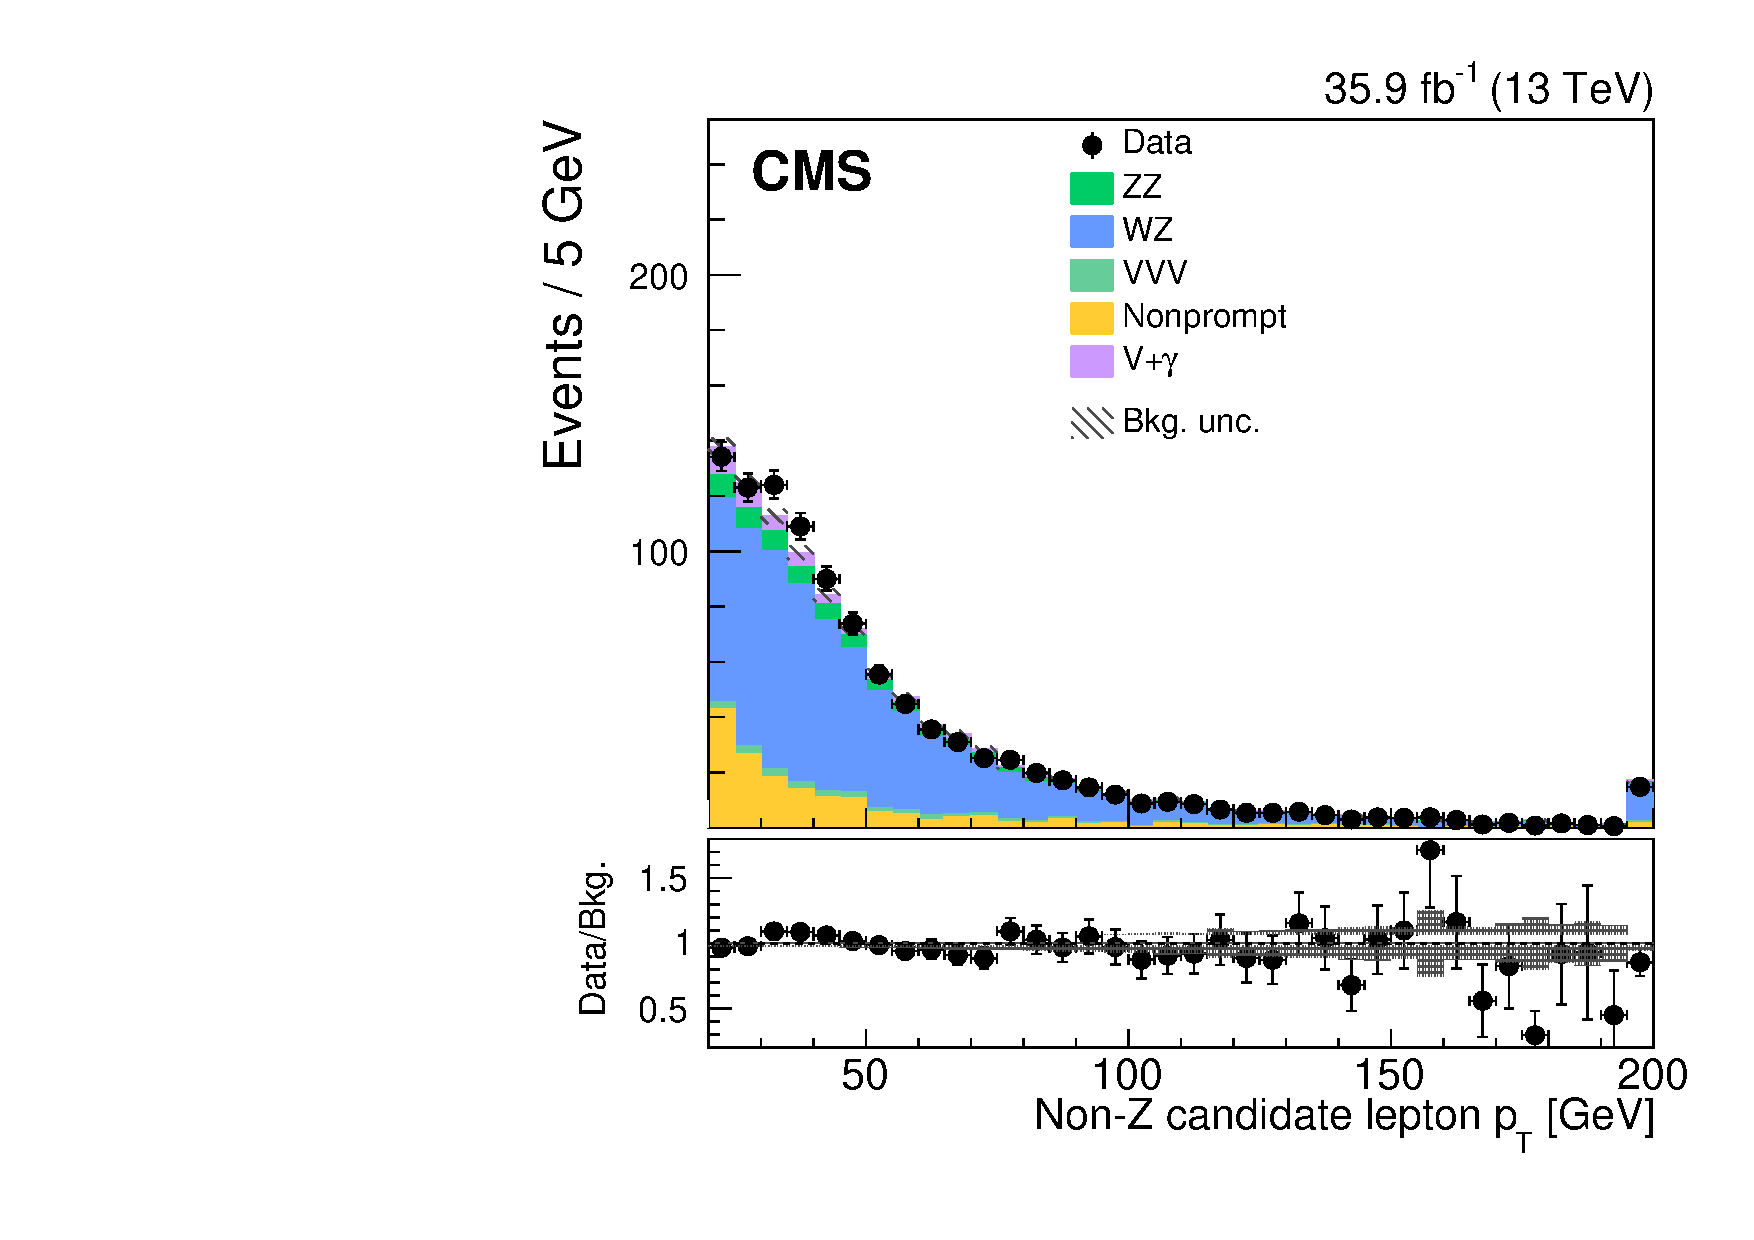
\includegraphics[width=0.48\textwidth]{figures/dibosons/wz3l/lepWpT_Nminus1.pdf}
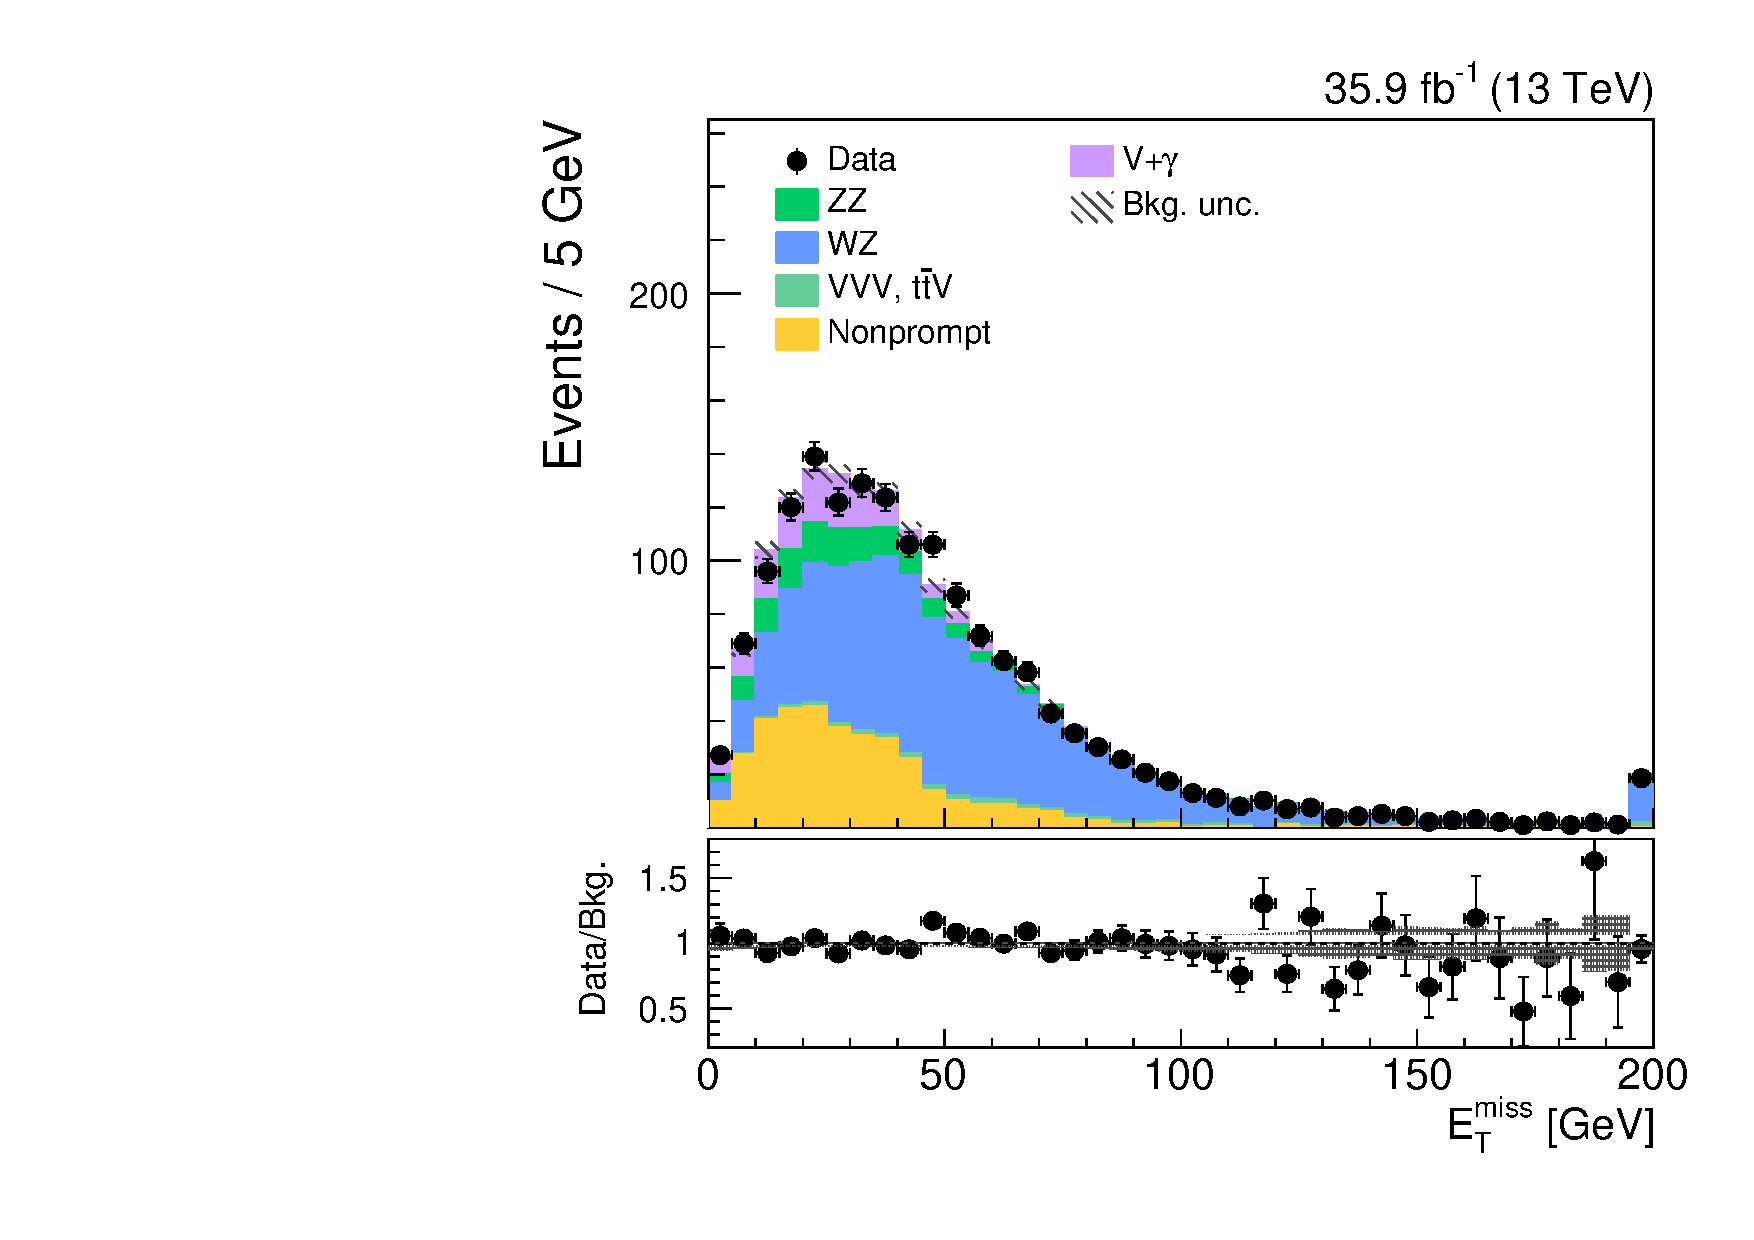
\includegraphics[width=0.48\textwidth]{figures/dibosons/wz3l/met_Nminus1.pdf}
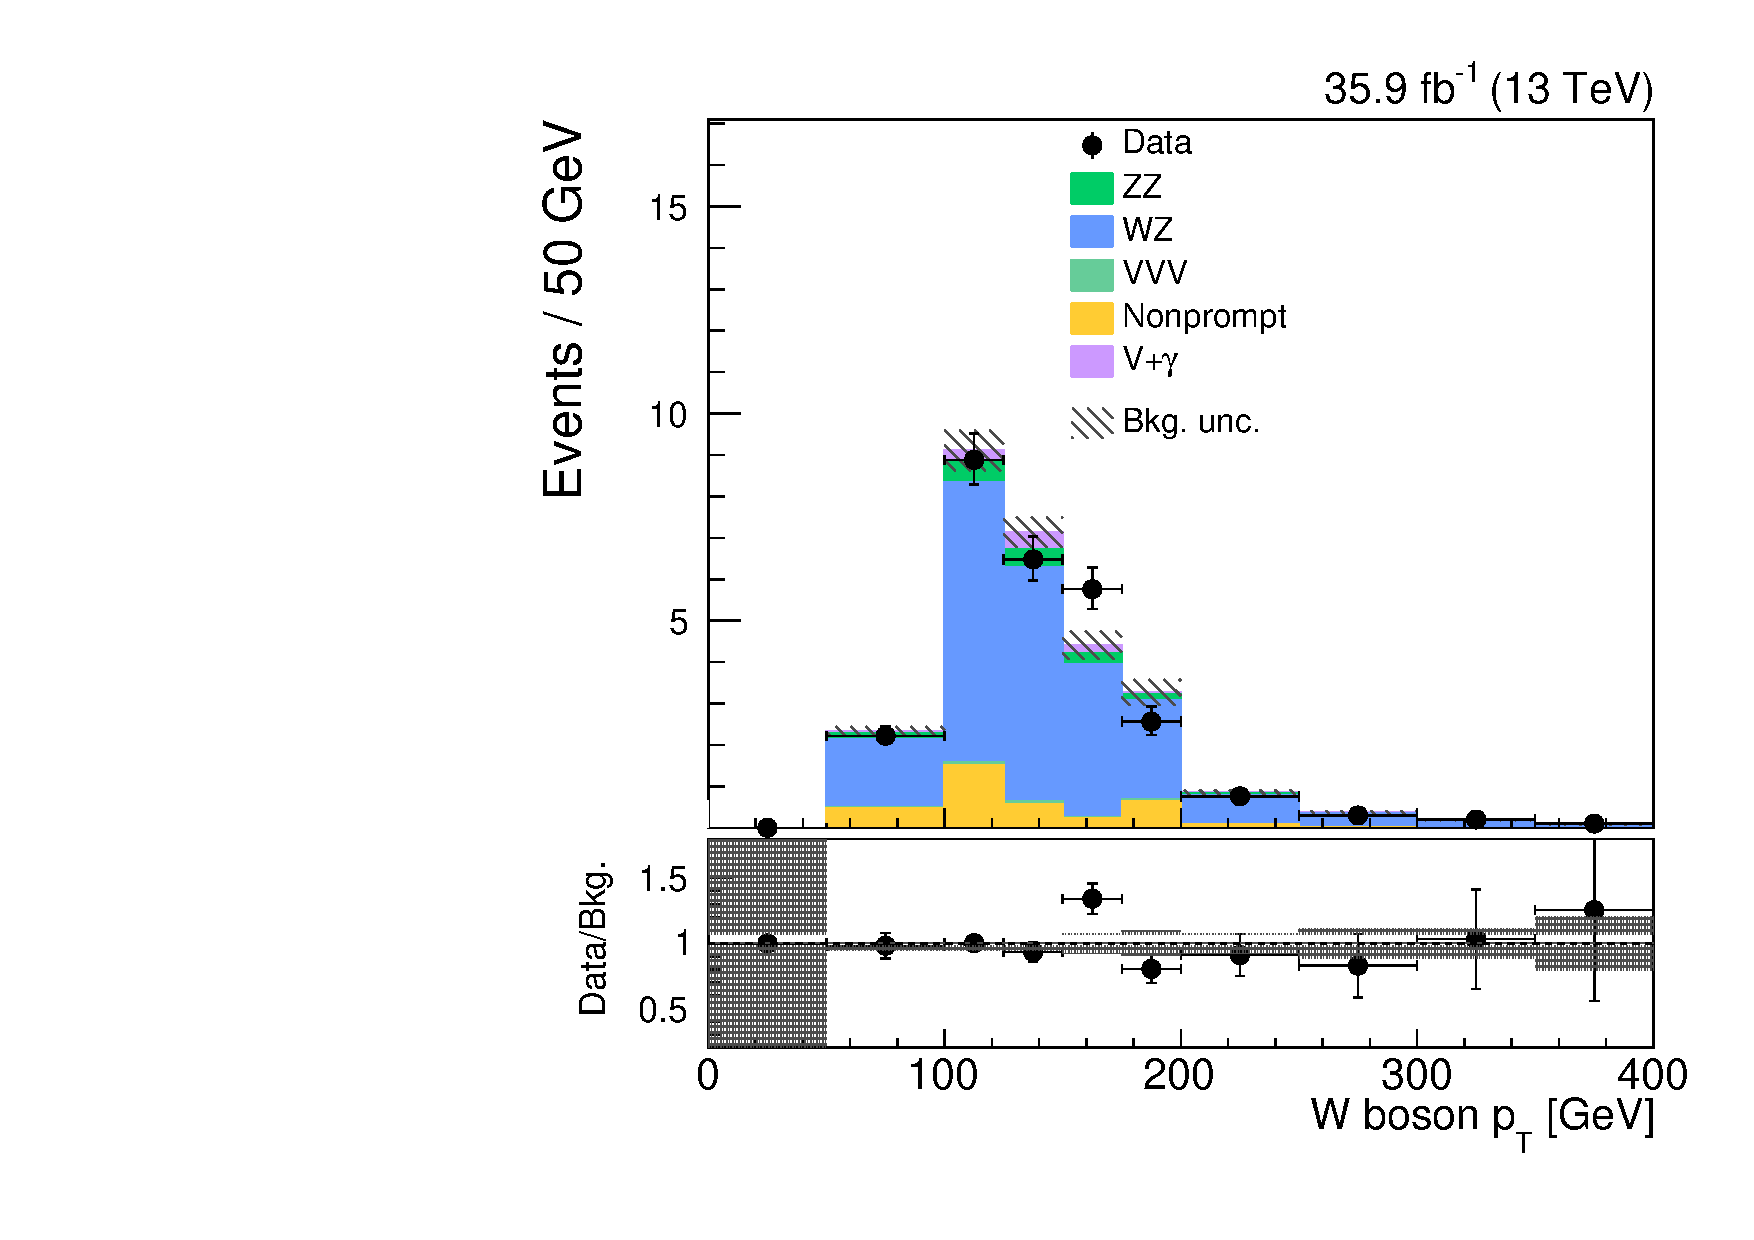
\includegraphics[width=0.48\textwidth]{figures/dibosons/wz3l/pTW.pdf}
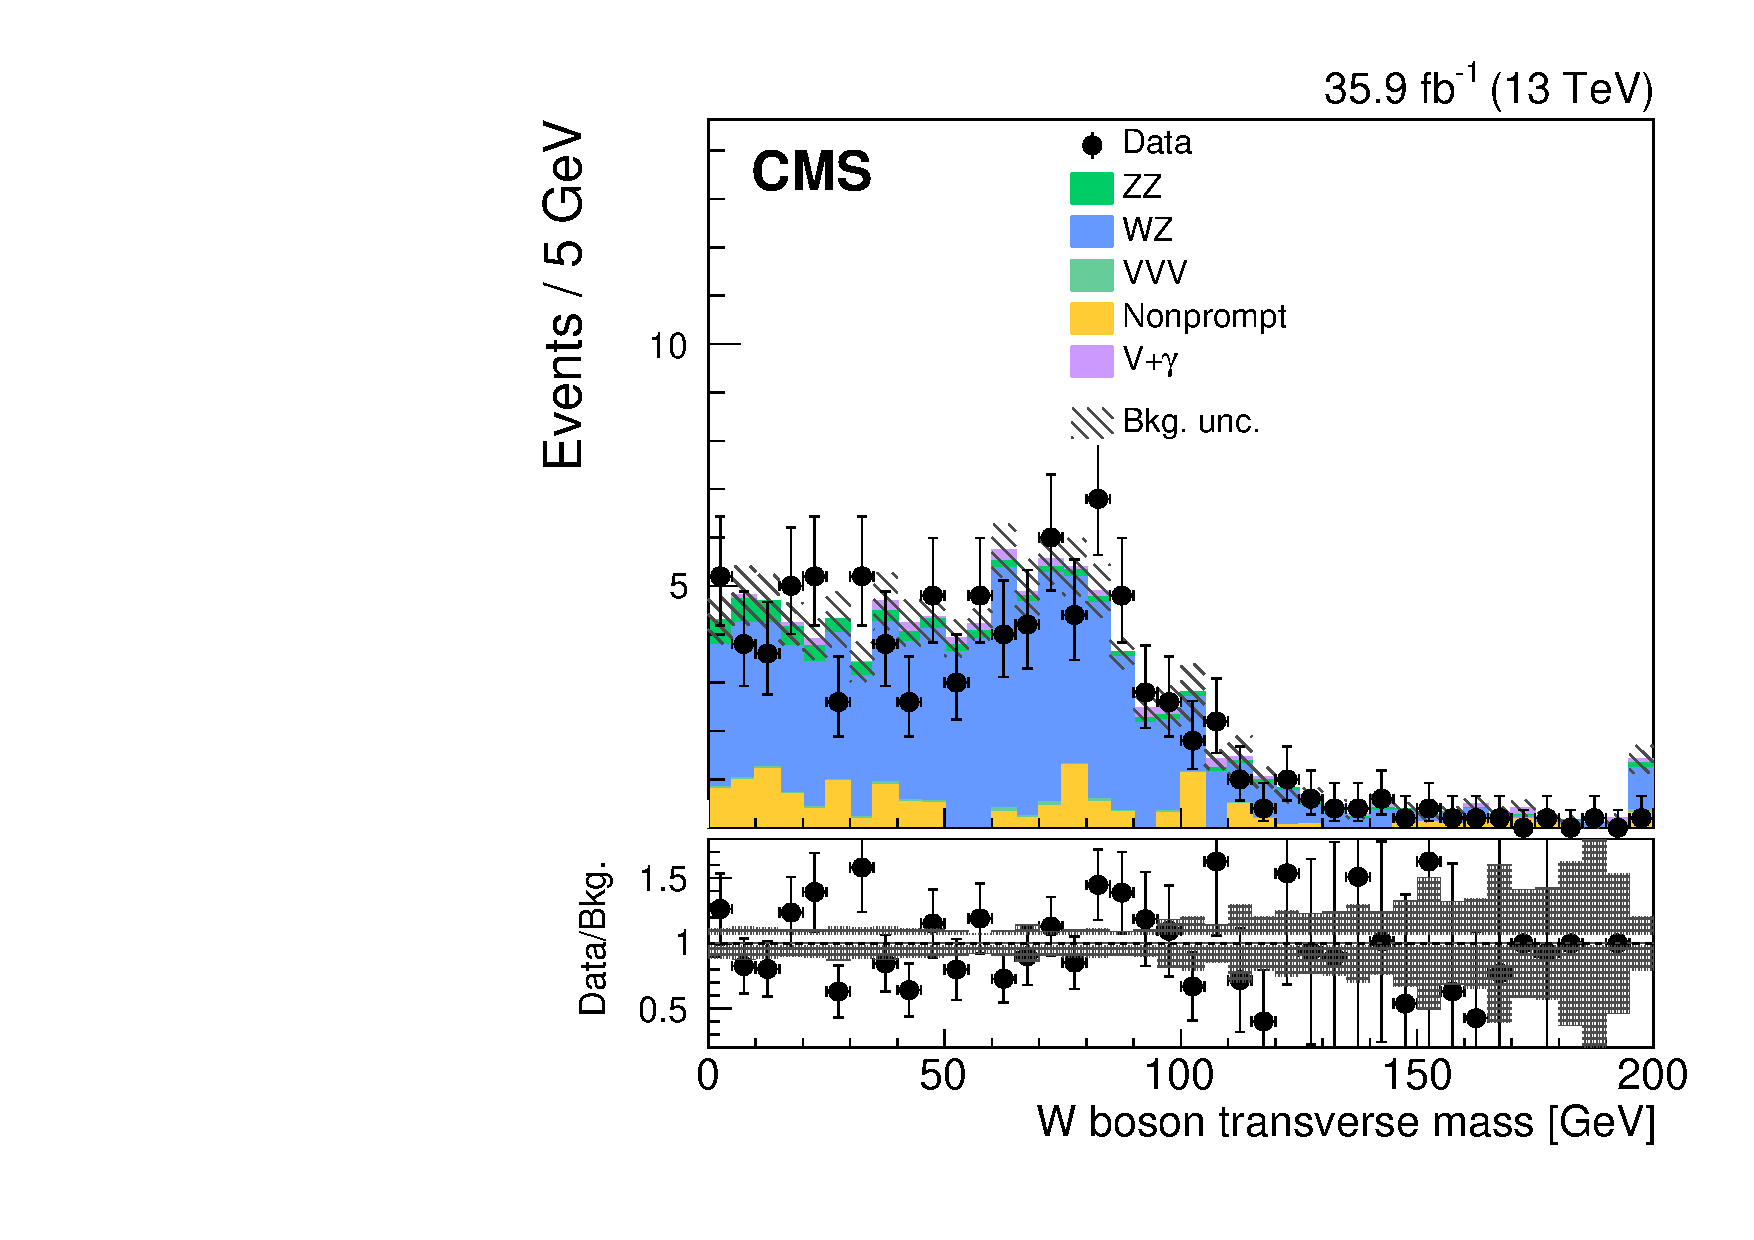
\includegraphics[width=0.48\textwidth]{figures/dibosons/wz3l/mTW.pdf}
\caption{Kinematics of the reconstructed W boson at final selection level. Clockwise from upper left: 
$p_\mathrm{T}$ of the lepton associated with the W boson;
$\met$ in the event; transverse mass of the W boson;
and $p_\mathrm{T}$ of the W boson.
Note the Jacobian peak in the transverse mass distribution.
The last bin includes the overflow events.
\label{fig:wz3l_w}}
\end{figure}





